%
\documentclass[preprint,12pt,authoryear]{elsarticle}

%% Use the option review to obtain double line spacing
% \documentclass[authoryear,preprint,review,12pt]{elsarticle}

%% Use the options 1p,twocolumn; 3p; 3p,twocolumn; 5p; or 5p,twocolumn
%% for a journal layout:
%% \documentclass[final,1p,times,authoryear]{elsarticle}
%% \documentclass[final,1p,times,twocolumn,authoryear]{elsarticle}
%% \documentclass[final,3p,times,authoryear]{elsarticle}
%% \documentclass[final,3p,times,twocolumn,authoryear]{elsarticle}
%% \documentclass[final,5p,times,authoryear]{elsarticle}
%% \documentclass[final,5p,times,twocolumn,authoryear]{elsarticle}

%% For including figures, graphicx.sty has been loaded in
%% elsarticle.cls. If you prefer to use the old commands
%% please give \usepackage{epsfig}

%% The amssymb package provides various useful mathematical symbols
\usepackage{amssymb}
%% The amsmath package provides various useful equation environments.
\usepackage{amsmath}
%% The amsthm package provides extended theorem environments
% \usepackage{amsthm}

% Pseudocode
\usepackage{algorithm}
\usepackage{algorithmic}

%% The lineno packages adds line numbers. Start line numbering with
%% \begin{linenumbers}, end it with \end{linenumbers}. Or switch it on
%% for the whole article with \linenumbers.
%% \usepackage{lineno}

\usepackage{array}

% \usepackage[colorlinks=true, allcolors=blue]{hyperref}
\usepackage[colorlinks=true, linkcolor=blue, citecolor=blue, urlcolor=blue]{hyperref}

\journal{Nuclear Physics B}

\begin{document}

\begin{frontmatter}

%% Title, authors and addresses

%% use the tnoteref command within \title for footnotes;
%% use the tnotetext command for theassociated footnote;
%% use the fnref command within \author or \affiliation for footnotes;
%% use the fntext command for theassociated footnote;
%% use the corref command within \author for corresponding author footnotes;
%% use the cortext command for theassociated footnote;
%% use the ead command for the email address,
%% and the form \ead[url] for the home page:
%% \title{Title\tnoteref{label1}}
%% \tnotetext[label1]{}
%% \author{Name\corref{cor1}\fnref{label2}}
%% \ead{email address}
%% \ead[url]{home page}
%% \fntext[label2]{}
%% \cortext[cor1]{}
%% \affiliation{organization={},
%%            addressline={}, 
%%            city={},
%%            postcode={}, 
%%            state={},
%%            country={}}
%% \fntext[label3]{}

\title{NOTE and T-NOTE an efficient transformer encoder for IoT task offloading in edge-fog-cloud computing environment
} %% Article title

%% use optional labels to link authors explicitly to addresses:
%% \author[label1,label2]{}
%% \affiliation[label1]{organization={},
%%             addressline={},
%%             city={},
%%             postcode={},
%%             state={},
%%             country={}}
%%
%% \affiliation[label2]{organization={},
%%             addressline={},
%%             city={},
%%             postcode={},
%%             state={},
%%             country={}}

\author{} %% Author name

%% Author affiliation
\affiliation{organization={},%Department and Organization
            addressline={}, 
            city={},
            postcode={}, 
            state={},
            country={}}

%% Abstract
\begin{abstract}
%% Text of abstract
Abstract text.
\end{abstract}

%%Graphical abstract
\begin{graphicalabstract}
%\includegraphics{grabs}
\end{graphicalabstract}

%%Research highlights
\begin{highlights}
\item Research highlight 1
\item Research highlight 2
\end{highlights}

%% Keywords
\begin{keyword}
%% keywords here, in the form: keyword \sep keyword

%% PACS codes here, in the form: \PACS code \sep code

%% MSC codes here, in the form: \MSC code \sep code
%% or \MSC[2008] code \sep code (2000 is the default)

\end{keyword}

\end{frontmatter}

%% Add \usepackage{lineno} before \begin{document} and uncomment 
%% following line to enable line numbers
%% \linenumbers

%% main text
%%

\section{Introduction}\label{sec:introduction}

\subsection{Background and motivation}\label{subsec:background}

The Internet of Things (IoT) has become a foundational element of modern technology, facilitating the development of innovative applications in domains such as smart cities, healthcare, autonomous systems, and other fields. The proliferation of IoT devices has been rapid and significant, with Cisco reporting a global total exceeding 30 billion~\citep{benaboura_comprehensive_nodate}. These devices generate a substantial volume of data, approximately 2 exabytes on a daily basis. Achieving maximum potential from these systems necessitates the implementation of efficient processing and analysis methodologies. This requirement presents a formidable challenge in the domains of data management, resource allocation, and system scalability.

The inherent limitations of IoT devices, such as their small batteries, limited processing power, and minimal storage capacity, render them ill-suited to manage the substantial volumes of data they generate. It is evident that tasks such as real-time processing of sensor data or computation-intensive applications frequently exceed the capabilities of local devices. Conventional approaches entail the delegation of these tasks to centralized cloud servers. However, network limitations and latency sensitivity frequently render this approach inefficient, particularly for real-time applications~\citep{benaboura_comprehensive_nodate}.

In order to address these challenges, fog computing has emerged as a distributed computing paradigm that extends the capabilities of cloud computing to the edge of the network. By facilitating the execution of storage, computation, and data management operations in close proximity to the data source, fog computing contributes to the reduction of latency, power consumption, and network traffic. It is evident that contemporary applications, including but not limited to smart homes, autonomous vehicles, smart agriculture, and healthcare, are contingent on this paradigm in order to satisfy their real-time and location-aware processing requirements as evoked by~\cite{das_review_2023}. Fog computing, first introduced in 2012, provides a hierarchical architecture that serves to bridge the gap between cloud servers and IoT devices, thereby allowing for seamless data flow and operational efficiency~\citep{fahimullah_review_2022}.

Notwithstanding the advantages inherent in task offloading in fog computing, this process is encumbered by numerous challenges. Optimizing resource utilization, reducing energy consumption, and maintaining Quality of Service (QoS) require robust strategies due to the heterogeneous and dynamic nature of fog networks. Factors such as fluctuating workloads, mobility, and task diversity have been identified as contributing to an increase in the complexity of the situation. In order to address these challenges, innovative resource allocation techniques are required, including Machine Learning-based (ML) methods, auction models, and heuristic optimization as~\cite{fahimullah_review_2022} exhibits.

Conventional resource management techniques frequently employ static heuristic approaches, which prove ineffective when confronted with the diverse and dynamic workloads that are characteristic of fog environments. These methods, when configured offline for specific scenarios, lack the scalability and flexibility required for real-time task offloading and resource optimization. Consequently, a substantial decline in performance is experienced as system demands increase~\citep{iftikhar_ai-based_2023}.

To address this problem, metaheuristics such as GA have emerged as powerful optimization techniques capable of handling the multi-objective nature of fog computing task offloading. GAs excel in exploring complex solution spaces and finding near-optimal trade-offs between conflicting objectives such as latency minimization, energy efficiency, and resource utilization. Unlike traditional optimization methods that often focus on single objectives, multi-objective genetic algorithms can simultaneously optimize multiple performance criteria, making them particularly suitable for fog computing environments where various QoS parameters must be balanced. The evolutionary nature of GAs allows them to adapt to dynamic network conditions and heterogeneous resource availability, providing robust solutions for real-time task offloading decisions.

Recent advancements in the field of Artificial Intelligence (AI), particularly deep reinforcement learning (DRL), have demonstrated considerable potential in addressing the intricacies of task offloading in fog environments. Research has demonstrated the efficacy of AI-driven approaches in reducing latency, energy consumption, and operational costs. As~\cite{fahimullah_review_2022} demonstrates in their review, techniques such as centralized Dueling Deep Q-Networks (DDQNs), decentralized learning models, and multi-agent reinforcement learning have been employed to optimize offloading policies and resource allocation. Furthermore, hybrid strategies that integrate artificial intelligence with conventional methods have demonstrated efficacy in heterogeneous fog environments~\citep{mishra_collaborative_2023}.

In order to maintain currency with the latest advancements in this domain, the present study investigates innovative methodologies that integrate the strengths of evolutionary computation and deep reinforcement learning for the purpose of optimizing IoT task offloading. The integration of these approaches addresses the limitations of individual techniques while leveraging their complementary advantages.


\subsection{Contributions}

To address these gaps, this work makes the following key contributions:
\begin{itemize} 
    \item The proposal of a two-transformers-based architecture, utilizing DQL for the purpose of task offloading within a cloud-fog-edge environment, is hereby presented. The selection of the node (edge, fog or cloud) to execute each incoming task is determined by these models, representing n different ctions. The NOTE system is oriented towards node-level features, such as CPU, buffer, and bandwidth. In contrast, the T-NOTE system incorporates additional task attributes, including size, deadline, and CPU-cycle requirements. This capability facilitates a more precise depiction of the interplay between node resources and task demands within a fog environment.

    \item This work also puts forth a model for offloading in hybrid environments that considers a substantial number of parameters for the QoS. To further expand upon the existing body of knowledge, an adaptation of a scenario with a real dataset was implemented within the framework of RayClousSim. We let open-source the scenario and the dataset for the community\footnote{\url{https://github.com/tutur90/Task-Offloading-Fog}}. All algorithms used, including NOTE and T-NOTE, are also implemented in this framework.

    \item Additionally, a comparative analysis was conducted between the GAs and a Deep Q-Learning (DQL) approach. The implementation of these algorithms in the training of a MLP constitutes a pivotal element of the study. The GA approach is employed in a dynamic setting, thereby enabling the MLP to be optimized for multi-objective offloading in real time.

\end{itemize}


\subsection{Paper organization}

The reminder of this paper is structured as follows: Section~\ref{sec:related_work} reviews related work; Section~\ref{sec:problem_modeling} describes the problem modeling, including the scenario and QoS modeling; Section~\ref{sec:offloading_strategies} details the proposed strategies, from genetics algorithm to deep reinforcement learning approaches, including Transformers-based methods; Section~\ref{sec:performance_evaluation} presents the experimental setup and results, as well as a comparative analysis of the proposed methods and that offloading analysis; finally, Section~\ref{sec:conclusion} concludes the paper and outlines future research directions.


\section{Related Work}\label{sec:related_work}


Task offloading in Fog/Cloud environments is a relatively recent research area compared to well-studied domains like image classification or time series forecasting. However, the decision-making process for task offloading is inherently complex due to its combinatorial nature.

\subsection{Deterministic Approaches}
Deterministic algorithms provide a direct method for solving the task offloading problem. For instance, the optimal task assignment algorithm proposed by Yan \textit{et al.}~\cite{yan_optimal_2020} employs a three-step approach: (i) assuming the offloading decisions are pre-determined, (ii) deriving closed-form expressions for optimal offloading, and (iii) implementing bisection search and a one-climb policy. This approach effectively reduces energy consumption and execution time for IoT tasks in Mobile Edge Computing (MEC) systems.

Nevertheless, the task offloading problem is considered NP-hard, as demonstrated in~\cite{guo_algorithmics_2024, jin_task_2024, sarkar_deep_2022}. Consequently, deterministic methods face scalability limitations, prompting the exploration of heuristic, metaheuristic, and AI-based approaches.


\subsection{Heuristic and Metaheuristic Methods}

Heuristic methods are well-suited for scaling in complex edge/cloud environments, as they avoid the exponential computational growth of deterministic algorithms \cite{zhang_survey_2024}. For example, the Deadline and Priority-aware Task Offloading (DPTO) algorithm \cite{adhikari_dpto_2020} schedules tasks by prioritizing delays and task priorities, selecting optimal devices to minimize overall offloading time.

Metaheuristic algorithms, known for their adaptability, have also shown strong performance.~\citep{bernard_d-npga_2024} introduced the Drafting Niched Pareto Genetic Algorithm (D-NPGA), which optimizes task offloading decisions and improves makespan and cost efficiency for IoT tasks in fog/cloud systems.

More sophisticated methods use multiple approaches. For example, Energy-Efficient and Deadline-Aware Task Scheduling in Fog Computing (ETFC)~\cite{pakmehr_etfc_2024} employs a Support Vector Machine (SVM) to predict traffic on fog nodes and classify them as low- or high-traffic. Then, they use reinforcement learning (RL) on the low-traffic group and a non-dominated sorting genetic algorithm III (NSGA-III) on the high-traffic group to make the offloading decision. This allows both algorithms to perform better on adequate tasks.

Metaheuristic approaches have gained attention for their ability to address the NP-hard nature of the task offloading problem with flexibility and adaptability. A recent and comprehensive survey by~\cite{rahmani_optimizing_2025} reviewed a wide range of metaheuristic algorithms—including Genetic Algorithms (GA), Particle Swarm Optimization (PSO), Ant Colony Optimization (ACO), and Grey Wolf Optimizer (GWO)—applied to task offloading in IoT environments. The review identified key strengths of these methods in balancing latency, energy consumption, and cost efficiency across heterogeneous fog-edge-cloud infrastructures. Their taxonomy also distinguishes between evolutionary and swarm-based algorithms, showing that hybrid models are increasingly used to adapt to dynamic network conditions. Despite their strengths, the authors noted limitations in scalability and real-time adaptability—areas where AI and deep learning techniques, such as DRL or transformers, may provide an edge.


\subsection{AI Approaches}

Machine learning (ML) has recently demonstrated its efficacy in task offloading. For instance, decision tree classifiers\cite{suryadevara_energy_2021} determine whether tasks should be offloaded to the fog or cloud, resulting in reduced latency and energy consumption. Logistic regression models\cite{bukhari_intelligent_2022} have also been applied, estimating the probability of successful offloading by leveraging maximum likelihood estimation.

Deep learning (DL), a subset of ML, deserves special attention due to its notable advances across various fields. 

Basic deep neural networks (DNNs) have been applied to IoT offloading tasks, such as~\citet{sarkar_deep_2022}, where parallel DNNs optimize cost, energy consumption, and latency. However, deep reinforcement learning (DRL) is often preferred for its decision-making capabilities in dynamic environments.

For example, Jiang \textit{et al.}\cite{jiang_reinforcement_2021} utilized Deep Q-Learning (DQN) to identify optimal offloading policies and resource allocation strategies for user equipment in fog/cloud systems. Their approach combines a dueling deep Q-network for model pre-processing and a distributed deep Q-network for efficient task allocation.

Moreover, multi-agent DRL methods\cite{ren_deep_2021} have been employed to offload IoT tasks. Each IoT device trains its DRL model to select fog access points, followed by a greedy algorithm to determine cloud offloading. This approach demonstrates competitive performance in energy efficiency compared to exhaustive search and genetic algorithms.

Long Short-Term Memory (LSTM) networks, a type of recurrent neural network, are particularly suitable for the temporal dimensions of task offloading. Tu \textit{et al.}\cite{tu_task_2022} combined LSTM with DQN to predict task dynamics in real-time, leveraging observed edge network conditions and server load. This hybrid model significantly improved latency, offloading cost, and task throughput.

Transformers, known for their revolutionary impact on natural language processing (NLP), have also been adapted for task offloading. Gholipour \textit{et al.}\cite{gholipour_tpto_2023} proposed TPTO, a transformer-based framework with Proximal Policy Optimization (PPO). Their model encodes task dependencies using a transformer encoder and employs an actor-critic framework trained with PPO to generate probability distributions for offloading actions, achieving state-of-the-art results in edge computing environments.

While many existing offloading solutions rely on synthetic datasets and focus on Multi-access or Vehicular Edge Computing (MEC/VEC) scenarios~\cite{fahimullah_review_2022, tu_task_2022, gholipour_tpto_2023}, research specifically targeting fog computing remains limited. In particular, models such as Deep Neural Networks (DNNs)~\cite{sarkar_deep_2022} and Deep Q-Learning (DQL)~\cite{jiang_reinforcement_2021} have rarely been evaluated in realistic fog environments using real-world data.

Genetic Algorithms (GAs) are often static in nature, such as~\citet{bernard_d-npga_2024, pakmehr_etfc_2024}, meaning that they cannot be employed in real-time applications and can only converge through iterations on the same simulation environment where tasks and their order remain static. This characteristic makes them particularly complex to deploy in real-world applications where dynamic adaptation is required.

Transformer-based deep learning techniques remain poorly explored in this domain, despite being state-of-the-art in many fields. Some exploration efforts show promise; however, existing approaches often implement basic action spaces, such as TPTO~\cite{gholipour_tpto_2023}, which is designed with only two actions: offloading the task to the cloud or processing it on the edge.

Algorithms are referenced in the Table~\ref{tab:task_offloading_methods} with the method, the dataset type, the QoS evaluated, and the job type. Used QoS are referenced in the Table~\ref{table:qos_metrics} with their description.


\begin{table*}[h!]
\centering

\resizebox{\textwidth}{!}{%
\begin{tabular}{|l|l|l|l|l|l|l|l|}
\hline
\textbf{Paper} & \textbf{Method} & \textbf{Algorithm} & \textbf{Dataset} & \textbf{QoS} & \textbf{Type of Job} & \textbf{Environment} & \textbf{Tool} \\ \hline
~\cite{yan_optimal_2020} & Deterministic & Optimal Task Assignment & Real & E, ET & IoT tasks & MEC & NA \\ \hline
~\cite{adhikari_dpto_2020} & Heuristic & DPTO & Synthetic & QWT, D & IoT tasks & Cloud \& Fog & NA \\ \hline
~\cite{bernard_d-npga_2024} & Metaheuristic & D-NPGA & Synthetic & C, M & IoT tasks & Cloud \& Fog & Python \\ \hline
This work & Metaheuristic & NPGA/NSGA-II+MLP & Real & C, L, TTR & IoT tasks & Cloud \& Fog & Python, PyTorch \\ \hline
~\cite{pakmehr_etfc_2024} & AI, Metaheuristics & ETFC & C, E, L, DLV & Synthetic & IoT tasks & Fog & NA \\ \hline
~\cite{bukhari_intelligent_2022} & AI & Logistic Regression (LR) & Real & C, E, L & IoT tasks & Cloud \& Fog & Python, Matlab \\ \hline
~\cite{suryadevara_energy_2021} & AI & Decision Tree (DT) & Synthetic & E, L & IoT tasks & Cloud \& Fog & iFogSim \\ \hline
~\cite{sarkar_deep_2022} & AI & Deep Neural Network (DNN) & Synthetic & C, E, L & Mobile & Cloud \& Fog & iFogSim \\ \hline
~\cite{jiang_reinforcement_2021}& AI & Deep Q-Network (DQN) & Synthetic & E, L & Mobile & Cloud \& Fog & Python, Adam optimizer \\ \hline
~\cite{ren_deep_2021} & AI & Multi-agent DRL & Synthetic & E & IoT tasks & Cloud \& Fog & NA \\ \hline
~\cite{tu_task_2022} & AI & DRL+LSTM & Real & C, L, TTR & Mobile & MEC & NA \\ \hline
~\cite{gholipour_tpto_2023} & AI & Transformers PPO & Synthetic & L & IoT tasks & Edge & Python, TensorFlow \\ \hline
This work & AI & DQL+MLP & Real & C, L, TTR & IoT tasks & Cloud \& Fog & Python, PyTorch \\ \hline
This work & AI & Transformers & Real & C, L, TTR & IoT tasks & Cloud \& Fog & Python, PyTorch \\ \hline
\end{tabular}
}
\caption{Summary of Task Offloading Methods in Fog and Edge Computing}\label{tab:task_offloading_methods}
\end{table*}


\begin{table*}[h]
\centering
\resizebox{\textwidth}{!}{%
\begin{tabular}{ |c|l| }
\hline
\textbf{Metric} & \textbf{Description} \\ \hline
C\@: Cost & Refers to the expenses incurred in task offloading, including computation, storage, and data transfer costs. \\ \hline
L\@: Latency & The time delay between the initiation of a request and the reception of the response. Crucial for real-time applications. \\ \hline
E\@: Energy & The total energy consumed during task offloading, including device and network-level energy usage. \\ \hline
ET\@: Execution Time & The total time taken to execute a task from start to finish, including computation and communication time. \\ \hline
D\@: Delay & The time difference between task submission and the start of its processing. Includes network and processing delays. \\ \hline
M\@: Makespan & The total time required to complete all tasks in a batch or workflow. Indicates overall system efficiency. \\ \hline
QWT\@: Queue Waiting Time & The duration a task spends waiting in the queue before being processed. Impacts response time and throughput. \\ \hline
TTR\@: Task Throw Rate & The rate at which tasks are successfully processed and completed in the system, indicating system throughput. \\ \hline
DLV\@: Dead Line Violation & The percentage or rate of tasks that succeed to complete within their specified deadlines, indicating system reliability and quality of service. \\ \hline
\end{tabular}
}
\caption{Explanation of QoS Metrics in Edge-Fog-Cloud Computing}\label{table:qos_metrics}
\end{table*}


\section{Problem Modeling}\label{sec:problem_modeling}

\subsection{Scenario Modeling}\label{sec:scenario_modeling}

This scenario is modeled according to foundational concepts presented in\cite{aazam_cloud_2022, bukhari_intelligent_2022, jazayeri_autonomous_2021}, following a three-tier offloading approach that involves \textit{edge}, \textit{fog}, and \textit{cloud} nodes. In Figure~\ref{fig:cloud-architecture}, a high-level cloud-enabled architecture is shown, where a Global Gateway (GG) collects tasks from various IoT devices before determining whether to process them locally or offload them to fog or cloud resources.


A real-world dataset of IoT-generated tasks, is employed to study and evaluate these offloading decisions. The tasks in this dataset vary in size, deadline constraints, and computational complexity, thereby reflecting the heterogeneous nature of practical IoT workloads.

\begin{figure}[ht]
    \centering
    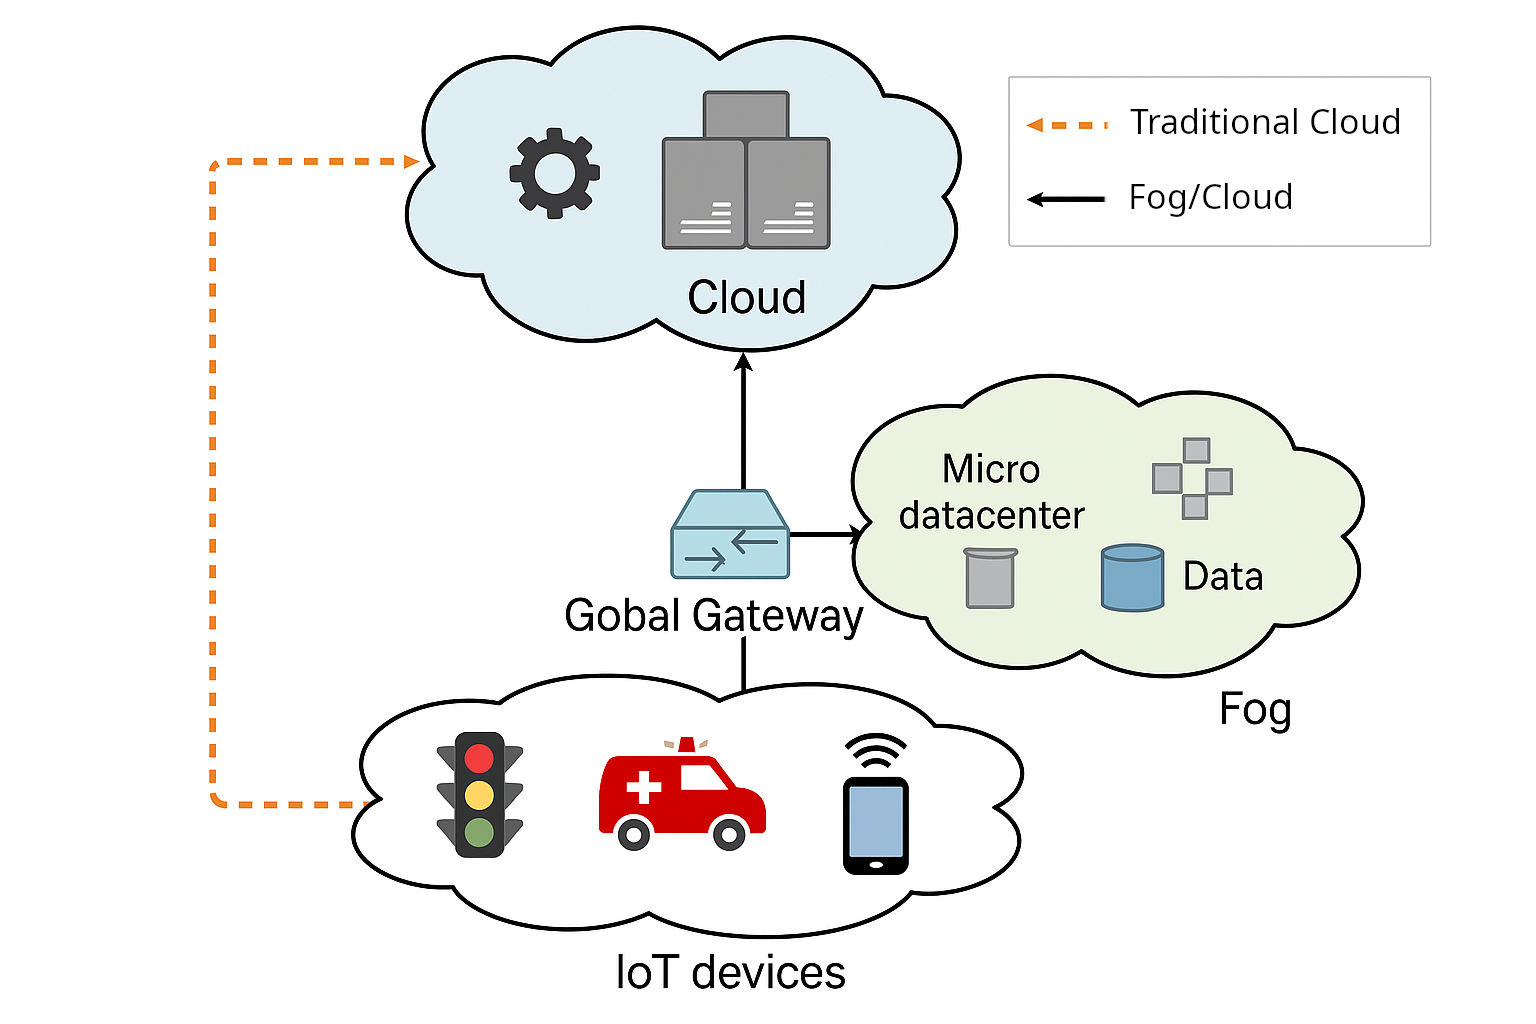
\includegraphics[width=0.75\linewidth]{figs/cloud_architecture.png}
    \caption{System Architecture}\label{fig:cloud-architecture}
\end{figure}


\subsubsection{Architecture}\label{subsec:architecture}

In Figure~\ref{fig:cloud-architecture}, a schematic overview of the proposed three-tier architecture is illustrated. The system is composed of IoT devices (sensors, mobile nodes, and other edge devices) that generate tasks. These tasks subsequently reach the Global Gateway, which processes them locally if resources are available, or decides to offload them to the fog or the cloud based on resource availability and energy considerations.

\paragraph{Global Gateway}\label{subsubsec:GG}

The GG layer is located at the edge and aggregates tasks from local IoT devices. In addition to routing capabilities, the GG has limited computational power, enabling it to handle smaller tasks locally and thus reduce network traffic. This approach is particularly advantageous for time-sensitive tasks that can be processed quickly on-site.

Upon receiving a task, several factors are evaluated:
\begin{itemize}
    \item Node state: The current load on the GG, along with the availability of fog and cloud nodes.
    \item Network conditions: Bandwidth, potential congestion, and latency to fog or cloud nodes.
    \item Energy usage: A predictive assessment of energy costs if the task is executed locally versus offloaded.
    \item Task requirements: Size, computational complexity, and deadline or QoS constraints.
\end{itemize}

A subsequent decision is made to determine the optimal execution strategy for the task. The system evaluates three primary options: processing the task locally if it is computationally feasible and resource-efficient, offloading the task to a nearby Fog Node to leverage edge computing capabilities, or offloading the task directly to a Cloud Node for intensive computational requirements that exceed local and fog node capacities.


\paragraph{Fog Nodes}\label{subsubsec:Fog}
Fog nodes provide moderate computational resources that exceed those of edge devices but remain below the capacity of cloud data centers. These intermediate computing nodes offer lower latency than distant cloud nodes due to their closer physical proximity to the network edge. Fog nodes serve as an essential intermediate tier for tasks that cannot be processed locally at the Gateway (GG) yet do not require the extensive resources of the cloud infrastructure. This positioning makes them ideal for applications requiring balanced performance between computational capability and response time.

\paragraph{Cloud Nodes}\label{subsubsec:Cloud}
Cloud nodes represent large-scale data centers with substantial computational and storage capabilities. Although they typically have higher baseline latencies because of greater network distances, they are well suited for computationally intensive applications. Cloud nodes excel in handling large tasks that demand significant CPU and memory resources, making them optimal for complex analytical workloads. They are particularly effective for batch processing scenarios with relaxed real-time constraints, where throughput is prioritized over immediate response. Furthermore, cloud data centers can accommodate high concurrency situations through dynamic resource scaling, allowing them to adapt to varying computational demands efficiently.

CPU capacity: Cloud servers can support a high volume of CPU cycles, facilitating efficient offloading for tasks with elevated computational demands.

\subsection{QoS Modeling}\label{sec:qos_modeling}

Task offloading decisions are evaluated within the RayCloudSim framework developed by~\cite{zhang2022osttd}, a comprehensive simulation platform for modeling and assessing cloud-edge-IoT computing environments based on LEAF~\citep{WiesnerThamsen_LEAF_2021}.

\subsubsection{Task Throw Rate}\label{subsubsec:task_throw_rate}

In distributed environments, task execution failures can occur due to issues such as \emph{network disconnections}, \emph{node isolation}, or \emph{buffer overflows}.

The \emph{task throw rate} \(\tau\) is defined as:
\begin{equation}
\tau = \frac{\text{Number of failed tasks}}{\text{Total tasks generated}}.
\end{equation}
A lower throw rate is indicative of a more robust and efficient offloading strategy.

\subsubsection{Latency}\label{subsubsec:latency}

The latency metric for task offloading is exclusively defined for tasks that achieve successful offloading, as the underlying assumption requires that tasks both arrive at the destination and undergo computational processing. For tasks meeting this criterion, the total latency encompasses three distinct components and is formally expressed as:
\begin{equation}
L_{\text{total}} = L_{\text{transmission}} + L_{\text{processing}} + L_{\text{queuing}}
\end{equation}
Conversely, for tasks that fail to achieve successful offloading, whether due to transmission failures, processing errors, or other system constraints, the total latency is assigned a null value:
\begin{equation}
L_{\text{total}} = 0
\end{equation}

\paragraph{Transmission Delay}
Transmission delay is composed of transfer delay and propagation delay:
\begin{equation}
L_{\text{transmission}} = L_{\text{transfer}} + L_{\text{propagation}}.
\end{equation}

\begin{enumerate}
    \item Transfer Delay: The duration required to send all bits of a packet onto the transmission medium:
    \begin{equation}
    L_{\text{transfer}} = \frac{S}{B},
    \end{equation}
    where \( S \) is the data size (in bits) and \( B \) is the allocated bandwidth for the task (in bits per second).

    \item Propagation Delay: The time taken for a signal to traverse the medium:
    \begin{equation}
    L_{\text{propagation}} = \frac{d}{v},
    \end{equation}
    where \( d \) is the total transmission distance (in meters) and \( v \approx 2 \times 10^8 \,\text{m/s}\) in optical fiber.
\end{enumerate}

\paragraph{Processing Delay}
Processing delay is the time spent by a computing node on executing a task:
\begin{equation}
L_{\text{processing}} = \frac{C \cdot S}{f},
\end{equation}
where \( C \) is the number of CPU cycles required to process the task, and \( f \) is the CPU frequency (in cycles per second).

\paragraph{Queuing Delay}
Queuing delay captures the waiting time a task experiences when the node is busy executing other tasks:
\begin{equation}
L_{\text{queuing}} = \sum_{i=1}^{N} L_{\text{processing}, i},
\end{equation}
where \( N \) is the number of tasks that arrived before the current task, and \( L_{\text{processing}, i} \) is the processing time of each task in the queue.

\subsubsection{Energy Consumption Model}\label{subsec:energy_consumption}

Similar to the latency metric, energy consumption is exclusively defined for tasks that achieve successful offloading. The simulation framework categorizes energy consumption into three distinct components:

\begin{itemize}
    \item \textbf{Idle Energy} $(E_{\text{idle}}^{i})$: Energy drawn by node $i$ when it remains idle, estimated through an idle power coefficient $P_{\text{idle}}$.
    \item \textbf{Execution Energy} $(E_{\text{exe}}^{i,k})$: Energy consumed by node $i$ during the execution of task $k$, based on execution power $P_{\text{exe}}$.
    \item \textbf{Transmission Energy} $(E_{\text{trans}}^{i,k})$: Energy utilized to transmit task $k$ from source node $j$ to destination node $i$, determined by a per-bit cost $C^{m,n}$ on the communication link.
\end{itemize}

All energy terms are expressed in Joules (J), while power $(P)$ is measured in Watts (W). Let $N$ denote the number of nodes and $T$ represent the total number of tasks successfully offloaded. The overall energy consumption in the system is calculated as:

\begin{equation}
E_{\text{total}} = 
    \sum_{i=1}^{N}
    \Bigl( E_{\text{idle}}^{i} + \sum_{k=1}^{T} 
    \bigl(E_{\text{exe}}^{i,k} + E_{\text{trans}}^{i,k}\bigr) \Bigr)
\end{equation}

This formulation ensures that energy consumption measurements reflect only the computational and communication activities associated with successful task offloading, maintaining consistency with the latency metric definition and providing a meaningful performance evaluation.

\paragraph{Node Power Consumption Model}
Based on the work of~\cite{ismail_computing_2021}, the power consumption of a computing node can be approximated by:
\begin{equation}
P(u_{\text{cpu}}) = \alpha + \beta \cdot u_{\text{cpu}},
\end{equation}
where:
\begin{itemize}
    \item \(\alpha\) represents the idle power \((P_{\text{idle}})\).
    \item \(\beta\) is the incremental power coefficient for executing tasks, defined by \(\beta = (P_{\text{exe}} - P_{\text{idle}})\).
    \item \(u_{\text{cpu}} \in [0,1]\) is the CPU utilization ratio.
\end{itemize}

This model has a Standard Error of Estimation (SEE) of 12.9\%, indicating a reasonably accurate fit to empirical data. 

\paragraph{Idle Energy}
The idle energy for node \(i\) over the entire simulation duration \(T\) can be calculated as:
\begin{equation}
E_{\text{idle}}^{i} = \int_{0}^{T} P_{\text{idle}}^{i} \, dt = P_{\text{idle}}^{i} \cdot T.
\end{equation}

\paragraph{Execution Energy}
Execution energy can be expressed by integrating the CPU utilization over time:
\begin{equation}
E_{\text{exe}}^{i} = \int_{0}^{T} \bigl(P_{\text{exe}}^{i} - P_{\text{idle}}^{i}\bigr) \cdot u_{\text{cpu}}(t) \, dt.
\end{equation}
In practical simulations, full CPU utilization \((u_{\text{cpu}} = 1)\) is often assumed while tasks are running, yielding:
\begin{equation}
E_{\text{exe}}^{i,k} = T_{\text{exe}}^{i,k} \cdot \bigl(P_{\text{exe}}^{i} - P_{\text{idle}}^{i}\bigr),
\end{equation}
where \(T_{\text{exe}}^{i,k}\) represents the execution time of task \(k\) on node \(i\).

\paragraph{Transmission Energy}
The transmission energy required to move task \(k\) from node \(j\) (source) to node \(i\) (destination) depends on data size and per-bit link costs:
\begin{equation}
E_{\text{trans}}^{i,k} = s^{k} \sum_{(m,n) \in I^{j,i}} C^{m,n},
\end{equation}
where:
\begin{itemize}
    \item \(s^{k}\) is the size of task \(k\) in bits.
    \item \(C^{m,n}\) is the energy cost per bit (J/bit) on the link from node \(m\) to node \(n\).
    \item \(I^{j,i}\) is the set of links used along the path from node \(j\) to node \(i\).
\end{itemize}

This model offers a structured, interpretable framework for quantifying energy consumption in offloading scenarios, thereby facilitating meaningful comparisons of energy efficiency under different scheduling and resource-allocation strategies.


\section{Proposed Offloading Strategies}\label{sec:offloading_strategies}


A range of offloading strategies was proposed to explore different decision-making paradigms, including NPGA, NSGA, and DQL. Each approach balances complexity and global optimality to varying degrees.

\subsection{Metaheuristics}\label{subsec:metaheuristics}

Metaheuristic algorithms, such as evolutionary methods, excel at exploring large, dynamic search spaces in IoT offloading. Although they have been applied in more static contexts by~\cite{bernard_d-npga_2024}, this work extends them to a \emph{dynamic} genome representation namely, an MLP mapping real-time states to offloading actions, following ideas proposed by~\cite{such2018deepneuroevolutiongeneticalgorithms}.

    

\subsubsection{GA}


\paragraph{Genome Representation (MLP Encoding)}
A candidate solution (or individual) is encoded as the set of weight matrices and bias vectors in a multi-layer perceptron (MLP). Each layer $\ell$ has trainable parameters $\mathbf{W}_\ell$ (weights) and $\mathbf{b}_\ell$ (bias). Thus, the full network is defined as
\[
\Big\{(\mathbf{W}_1, \mathbf{b}_1), (\mathbf{W}_2, \mathbf{b}_2), \dots, (\mathbf{W}_L, \mathbf{b}_L)\Big\}.
\]
These parameters determine how input features (e.g., CPU, buffer, bandwidth) are progressively transformed into node-specific scores for offloading. Evolutionary operators act directly on both the weight matrices and the bias vectors over multiple generations.

\paragraph{MLP Forward Mapping}
For an input feature vector $\mathbf{X}$, the MLP computes the output $\mathbf{Y}$ layer by layer:
\[
\mathbf{h}_1 = \phi(\mathbf{W}_1 \mathbf{X} + \mathbf{b}_1), \quad
\mathbf{h}_2 = \phi(\mathbf{W}_2 \mathbf{h}_1 + \mathbf{b}_2), \quad \dots \quad
\mathbf{Y} = f(\mathbf{W}_L \mathbf{h}_{L-1} + \mathbf{b}_L),
\]
where $\phi(\cdot)$ is a non-linear activation function (e.g., ReLU, sigmoid), and $f(\cdot)$ is the output activation (e.g., softmax for classification, linear for regression).

\paragraph{Crossover and Mutation}
\textbf{Crossover:} Two parent genomes
\(\{(\mathbf{W}_\ell^{(p1)}, \mathbf{b}_\ell^{(p1)})\}\) 
and 
\(\{(\mathbf{W}_\ell^{(p2)}, \mathbf{b}_\ell^{(p2)})\}\)
are combined by arithmetic crossover:
\[
\mathbf{W}_\ell^{(\text{child})} 
= \alpha\,\mathbf{W}_\ell^{(p1)} 
+ (1-\alpha)\,\mathbf{W}_\ell^{(p2)}, \qquad
\mathbf{b}_\ell^{(\text{child})} 
= \alpha\,\mathbf{b}_\ell^{(p1)} 
+ (1-\alpha)\,\mathbf{b}_\ell^{(p2)},
\]
where $\alpha \in [0,1]$ is chosen at random, ensuring offspring inherit traits from both parents.

\textbf{Mutation:} With probability $p_{\text{mutation}}$, each element of a weight matrix or bias vector is perturbed by Gaussian noise:
\[
\mathbf{W}[i,j] \leftarrow \mathbf{W}[i,j] + \epsilon_{ij}, 
\qquad 
\mathbf{b}[k] \leftarrow \mathbf{b}[k] + \delta_{k},
\]
where $\epsilon_{ij}, \delta_k \sim \mathcal{N}(0,\sigma^2)$. Clipping may be applied to maintain valid parameter ranges.


\paragraph{Overall Workflow of Genetic Algorithms}
The genetic algorithm process begins with population initialization, where an initial population of candidate solutions (chromosomes) is randomly generated using an appropriate representation format. Each individual in the population is then evaluated using multiple objective functions to determine fitness values across all optimization criteria. The selection phase follows, where parent individuals are chosen for reproduction based on their performance scores. The core evolutionary operations of crossover and mutation are then applied to generate offspring by recombining selected parents through crossover operations and introducing random variations through mutation. Subsequently, the replacement phase evaluates new offspring and forms the next generation by combining or replacing individuals from the parent and offspring populations using multi-objective replacement strategies. The algorithm terminates after reaching a maximum number of generations, achieving convergence criteria, or meeting other predefined stopping conditions. The final Pareto front represents the set of non-dominated solutions, effectively demonstrating the trade-offs among competing objectives. The pseudo code of the GA is referenced in Algorithm~\ref{alg:moega_iot_offloading}.

\paragraph{Multi-objective GA} As the GA algorithm is based on multiple individuals, it can achieve multiple objectives. During the selection process, the selected individuals were able to select multiple scores, rather than a single score, thereby creating the Pareto front. The present study focuses on two scalable and robust approaches. 

\emph{NPGA}~\citep{horn1994npga} employs a combination of tournament selection and a niching mechanism to maintain population diversity and prevent premature convergence to a single region of the Pareto front. The selection process works by conducting tournaments between randomly selected candidate solutions, where the winner is determined based on Pareto dominance relationships within a randomly chosen comparison set. Specifically, two candidates compete by counting how many individuals they dominate from a subset of the population, and the candidate with higher dominance count is selected. This approach naturally maintains diversity by distributing selection pressure across different regions of the Pareto front without requiring explicit front classification.

In contrast, \emph{NSGA-II}~\citep{Deb2002AFA} uses non-dominated sorting to classify solutions into hierarchical fronts and employs crowding distance calculations to preserve solution diversity within each front and guide selection for the next generation. The selection mechanism first performs non-dominated sorting to organize the population into ranked fronts ($\mathcal{F}_1, \mathcal{F}_2, \ldots$), where $\mathcal{F}_1$ contains the best non-dominated solutions. Within each front, crowding distance is calculated to measure the density of solutions in the objective space, favoring individuals in less crowded regions. Selection prioritizes individuals from better fronts first, and within the same front, those with larger crowding distances are preferred to maintain diversity along the Pareto front.


\begin{algorithm}[H]\label{alg:moega_iot_offloading}
\caption{Multi-Objective Genetic Algorithm for IoT Task Offloading}

\begin{algorithmic}[1]
\REQUIRE{Generations $G_{\max}$, population size $N$, crossover rate $p_c$, mutation rate $p_m$}
\ENSURE{Pareto-optimal offloading policies $\mathcal{P}^*$}

\STATE{Initialize population $\mathcal{P}_0$ with $N$ random MLP genomes}

\FOR{$g = 0$ to $G_{\max}-1$}
    \STATE{\textbf{Evaluate:} For each individual $\chi_i \in \mathcal{P}_g$}
    \STATE{\quad Simulate offloading with MLP weights from $\chi_i$}
    \STATE{\quad Compute objectives: $f_L$ (latency), $f_E$ (energy), $f_{TTR}$ (timeout rate)}

    \STATE{\textbf{Select:} Create mating pool $\mathcal{M}_g$ using multi-objective selection}
    \STATE{\quad (NSGA-II\: non-dominated sorting + crowding distance)}
    \STATE{\quad (NPGA\: Pareto tournament selection)}

    \STATE{\textbf{Reproduce:} Generate offspring $\mathcal{Q}_g$}
    \FOR{$i = 1$ to $N$}
        \STATE{Select parents $\chi_p, \chi_q$ from $\mathcal{M}_g$}
        \STATE{Apply crossover (prob. $p_c$) and mutation (prob. $p_m$)}
        \STATE{Add offspring to $\mathcal{Q}_g$}
    \ENDFOR{}

    \STATE{\textbf{Replace:} Form next generation $\mathcal{P}_{g+1}$ from $\mathcal{P}_g$ and $\mathcal{Q}_g$}
\ENDFOR{}

\RETURN{Non-dominated solutions from final population}
\end{algorithmic}
\end{algorithm}


\subsection{Deep Q-Learning}\label{subsec:DQL}

DQL is well-suited for IoT offloading because (i) the environment state (CPU, buffer, bandwidth, task attributes) evolves over time, (ii) each offloading decision alters subsequent states and tasks, and (iii) a reward can be assigned at each step (e.g., penalizing task failures or excessive latency).

\paragraph{Core Algorithm}
A neural network approximates the Q-function, estimating the long-term value of choosing an action (offloading to a particular node) in a given state. Training leverages mini-batches from an experience replay buffer of past transitions \((s,a,r,s')\). Iteratively, these Q-values converge, leading to improved decisions over time.

\paragraph{Workflow}
The DQL workflow, as detailed in Algorithm~\ref{alg:DQL_iot_offloading}, begins with initialization where an environment is built reflecting a specific scenario with fog/cloud nodes and tasks, an IoT task dataset is split into training/testing sets, and the neural network is configured with parameters such as hidden layers and learning rate. At each step, the agent constructs an observation by creating a flattened vector of node resources including free CPU, buffer, and link bandwidth, which the neural network uses to estimate Q-values for each node. Action selection follows an \(\varepsilon\)-greedy policy where with probability \(\varepsilon\), a random node is chosen for exploration, while otherwise the node with the highest Q-value is selected for exploitation. The environment is then updated as the chosen node processes the task, with the simulation advancing until the task completes or another event occurs such as queue filling or deadline miss, potentially causing task failure. Upon task completion or failure, a reward \(r\) is calculated and the transition \((s,a,r,s')\) is stored in the replay buffer, where the reward function is defined as:
\[
\textit{r} = 
\begin{cases}
\lambda_0, & \text{if task fails};\\[4pt]
\lambda_1 \,\dfrac{L_{\text{task}}}{\max(L_{\text{epoch}})} 
\;+\;
\lambda_2 \,\dfrac{E_{\text{task}}}{\max(E_{\text{epoch}})},
& \text{otherwise}.
\end{cases}
\]
Here, \(\lambda_0\) (often negative/zero) penalizes failure, \(L_{\text{task}}, E_{\text{task}}\) are normalized by epoch maxima, and \(\lambda_1, \lambda_2\) tune the importance of latency and energy, respectively. Finally, after a certain number of tasks, transitions are sampled from the replay buffer for training updates, where the Q-learning target is computed as \(Q_{\text{target}} = r \;+\; (1 - \mathbf{1}_{\text{done}})\,\gamma\, \max_{a'} Q(s',a')\), and the network is trained using methods such as MSE loss to align predicted Q-values with \(Q_{\text{target}}\), with Q-value estimates converging over multiple epochs.

\paragraph{Key Observations}
Several key observations emerge from the DQL approach. Failure penalties implemented through a negative \(\lambda_{0}\) can strongly discourage decisions that often cause task failures, providing a direct mechanism to avoid poor offloading choices. Metric normalization achieved by dividing latency and energy by epoch-wide maxima ensures bounded values for stable learning, preventing any single metric from dominating the reward signal. Metric emphasis can be adjusted by tuning \(\lambda_{1,2}\) to shift the balance between minimizing latency and saving energy, allowing the system to be configured for different optimization priorities. Finally, architectural flexibility is maintained since although an MLP is standard, more sophisticated models such as Transformers can replace or extend the MLP while retaining the same DQL pipeline.

\subsubsection{MLP-Based DQL}\label{subsubsec:mlp_DQL}
MLP-based DQL mirrors the MLP structure used in genetic algorithms, but instead of evolving weights, it trains them via Q-learning. The architecture consists of a feed-forward MLP that processes the current system state including CPU, buffer, bandwidth, and other relevant metrics, and outputs Q-values per node to guide the offloading decision. The policy employs an \(\varepsilon\)-greedy strategy that balances exploration and exploitation, ensuring the agent can discover new promising strategies while leveraging learned knowledge. The reward definition encodes latency, energy, and failures into a comprehensive reward function that captures the multi-objective nature of the offloading problem. Batch updates are performed by sampling from a replay buffer, which helps stabilize training and reduce correlation among transitions, leading to more robust learning dynamics.


\subsubsection{Transformer-based DQL}\label{subsubsec:transformers}

Transformer architectures~\citep{vaswani2023attentionneed} leverage multi-head self-attention to model complex relationships across various domains, despite often having high parameter counts. Task offloading is no exception, as shown by~\citet{gholipour_tpto_2023}, where a PPO-based policy was employed for Transformers. In the present work, two Transformer-based DQL variants are introduced to enable task offloading across multiple nodes:

\paragraph{NOTE}\label{par:note}

NOTE encodes each node’s available resources (CPU, buffer, and bidirectional link bandwidth) into an embedding vector. A positional encoding is then added to identify each node’s location in the topology. A Transformer encoder stack processes these node embeddings in parallel, enabling the model to learn both pairwise and global context. Finally, a feed-forward projection estimates the Q-value for each node, guiding the offloading decision. Because NOTE primarily targets node-level features, tasks are treated in an aggregated manner.

\begin{itemize}
    \item \textbf{Node Embeddings:} CPU frequency, buffer size, and upstream/downstream bandwidth are first passed through a fully connected layer to produce an embedding of dimension \(\displaystyle d_{\text{model}}\), where \(d_{\text{model}}\) is the hidden dimension of the model. Concatenating all node embeddings yields a tensor of size \(\displaystyle n_{\text{nodes}} \times d_{\text{model}}\), where \(n_{\text{nodes}}\) is the total number of nodes in the environment.
    \item \textbf{Positional Encoding:} Trainable parameters that characterize each node’s position in the network topology. These embeddings also form a \(\displaystyle n_{\text{nodes}} \times d_{\text{model}}\) matrix.
    \item \textbf{Transformer Encoder:} Multi-head self-attention highlights potential bottlenecks and optimal resource matches among the nodes. Residual connections and layer normalization are used, followed by a feed-forward sublayer with a GELU activation~\citep{hendrycks2023gaussianerrorlinearunits}. This encoder block is repeated \(N\) times.
    \item \textbf{Output Layer:} A fully connected layer projects the encoded representations to Q-values, producing one scalar per node. The node with the highest Q-value is then chosen for offloading.
\end{itemize}

\begin{figure}[H]
    \centering
    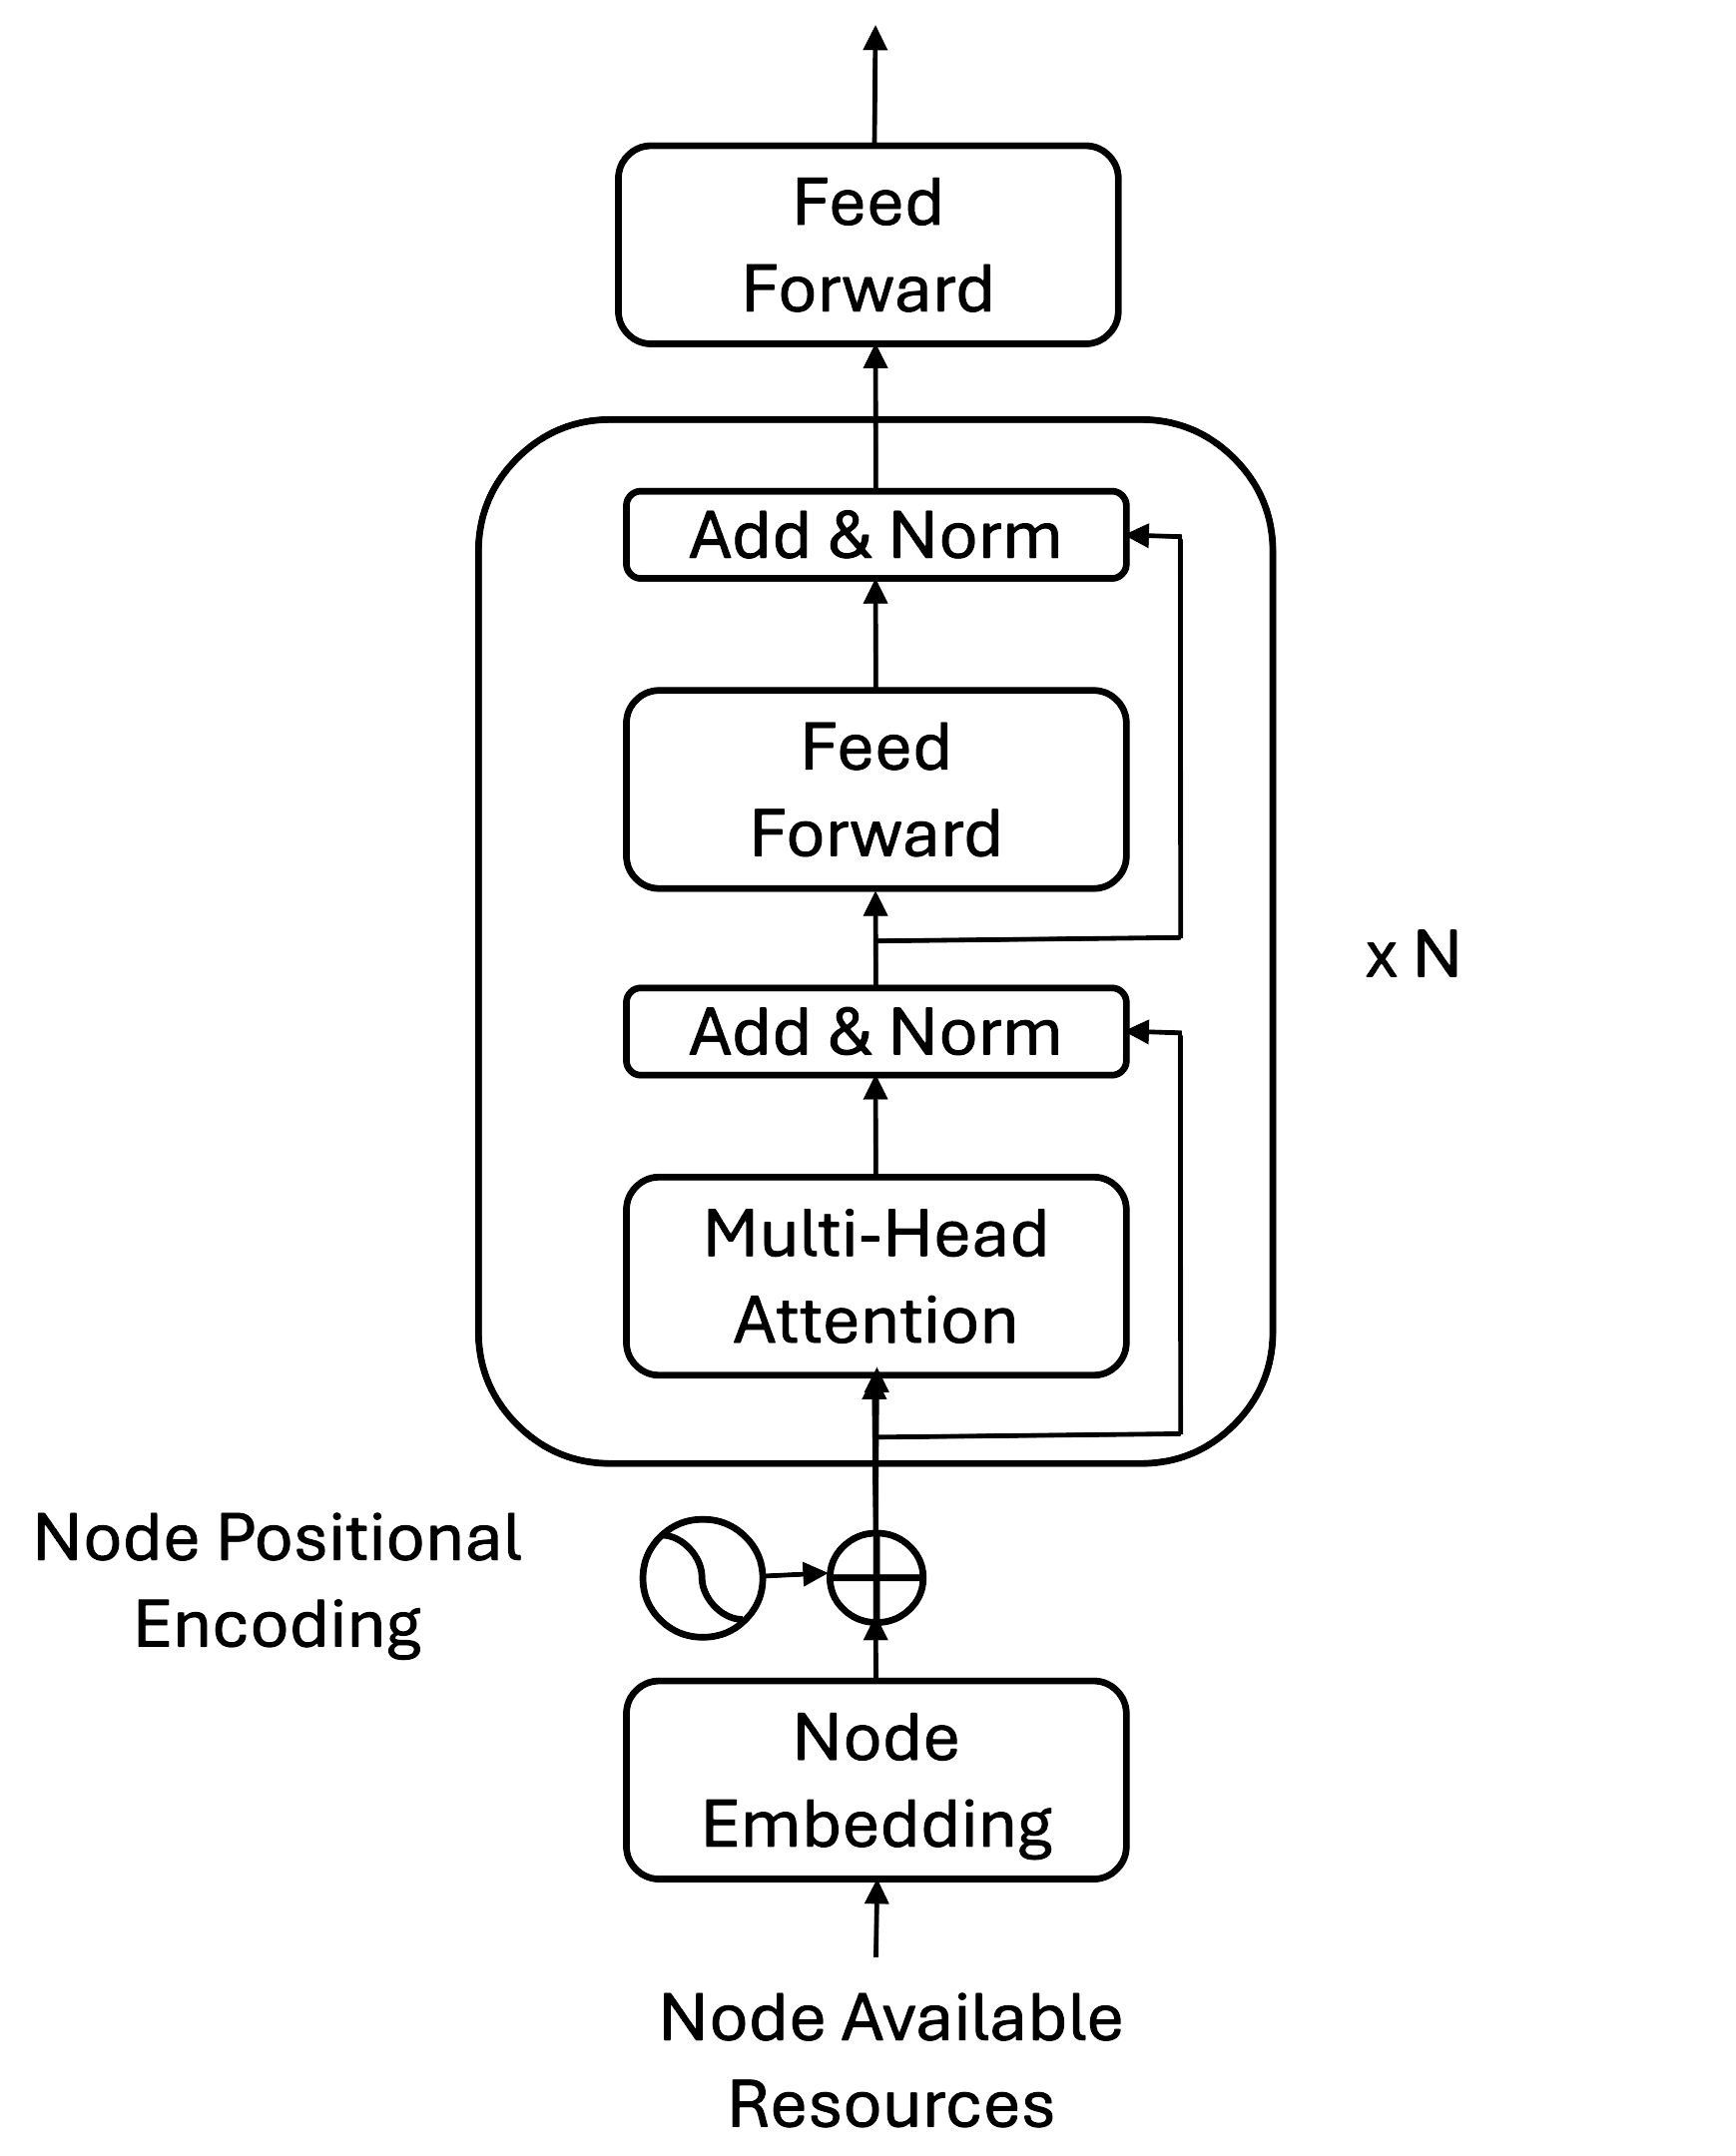
\includegraphics[width=0.6\linewidth]{figs/nodeformer_architecture.png}
    \caption{NOTE Architecture}\label{fig:note_architecture}
\end{figure}

\paragraph{T-NOTE}\label{par:T-NOTE}

T-NOTE extends NOTE by incorporating task attributes (e.g., size, deadline, and CPU-cycle requirements). These task features are passed through a fully connected layer to produce a vector of size \(d_{\text{model}}\). The resulting vector is then replicated across the \(n_{\text{nodes}}\) dimension and added to the node embeddings and node positional encodings before entering the Transformer encoder. Task-specific positional encoding can be combined or managed separately, allowing the model to capture task characteristics through shared attention. While including task information enables the Transformer encoder to more accurately learn interactions between node resources and task demands, it also increases the complexity of each DQL state. This added complexity sometimes leads to greater model instability, as rapid changes in the task dimension can cause oscillations in policy behavior. Consequently, NOTE (which omits explicit task embeddings) may remain advantageous in scenarios where a simpler, more stable representation is desired.


\begin{figure}[H]
    \centering
    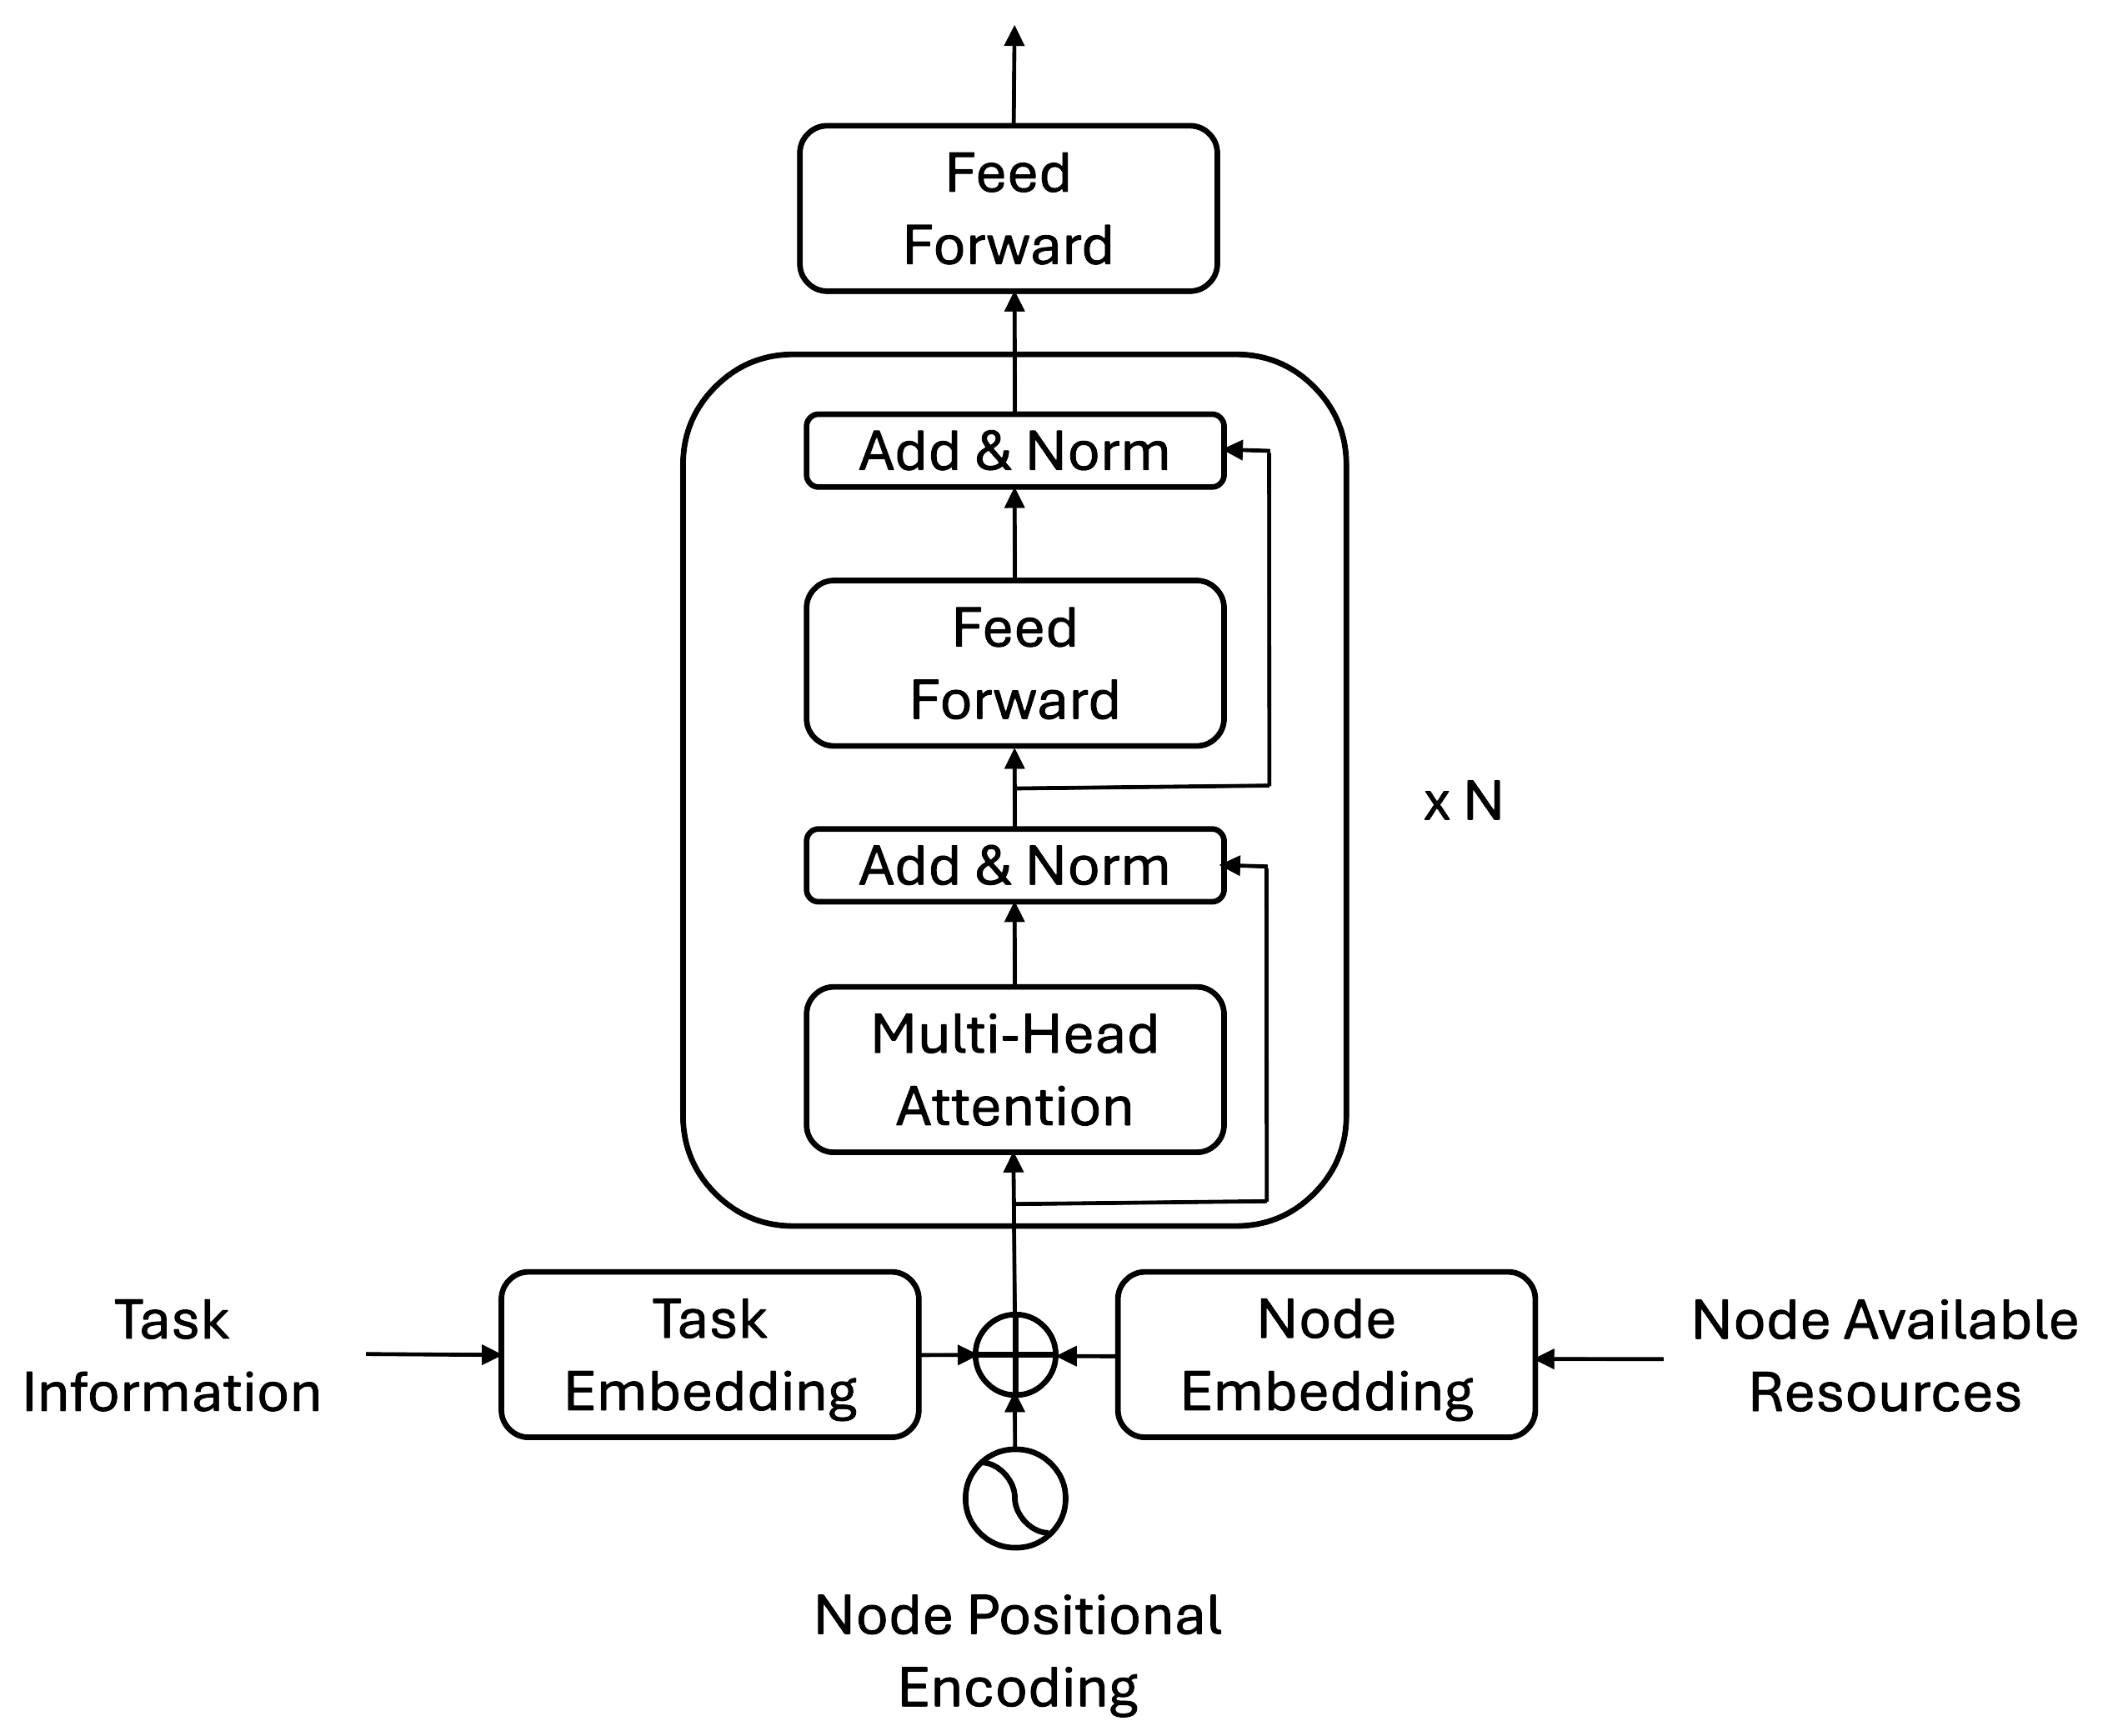
\includegraphics[width=0.8\linewidth]{figs/taskformer_architecture.png}
    \caption{T-NOTE Architecture}\label{fig:t-note_architecture}
\end{figure}


\begin{algorithm}[H]
\caption{Deep Q-Reinforcement Learning for IoT Task Offloading}\label{alg:DQL_iot_offloading}
\begin{algorithmic}[1]
\REQUIRE{Environment $\mathcal{E}$, task dataset $\mathcal{D}$, hyperparameters $\{\alpha, \gamma, \epsilon_0, \epsilon_{\text{decay}}, \lambda_0, \lambda_1, \lambda_2\}$}
\ENSURE{Trained Q-network policy $\pi^*$}

\STATE{Initialize Q-network $Q_\theta$ with random parameters $\theta$}
\STATE{Initialize experience replay buffer $\mathcal{B} \leftarrow \emptyset$}
\STATE{Set exploration rate $\epsilon \leftarrow \epsilon_0$}

\FOR{epoch $e = 1$ to $E_{\max}$}
    \STATE{Initialize epoch metrics: $L_{\max}^{(e)} \leftarrow 0$, $E_{\max}^{(e)} \leftarrow 0$}

    \FOR{each task $\tau_i \in \mathcal{D}$ ordered by generation time}
        \STATE{Wait until $t_{\text{current}} \geq \tau_i.\text{arrival\_time}$}
        \STATE{Construct state vector $s_i$ from system resources/task features}

        \STATE{\textbf{Action Selection:}} 
        \IF{$\text{rand}() < \epsilon$}
            \STATE{$a_i \leftarrow$ random edge node}
        \ELSE{}
            \STATE{$a_i \leftarrow \arg\max_{a} Q_\theta(s_i, a)$}
        \ENDIF{}
        
        \STATE{Execute offloading action $a_i$ and simulate task execution}
        \STATE{Observe next state $s_{i+1}$ and compute reward:}
        \STATE{
        \[
        r_i = \begin{cases}
        \lambda_0 & \text{if task execution fails} \\[0.5em]
        -\lambda_1 \cdot \frac{L_i}{L_{\max}^{(e)}} - \lambda_2 \cdot \frac{E_i}{E_{\max}^{(e)}} & \text{otherwise}
        \end{cases}
        \]
        }
        
        \STATE{Store transition $(s_i, a_i, r_i, s_{i+1})$ in $\mathcal{B}$}
        
        \IF{$|\mathcal{B}| \geq$ batch\_size \OR{} end of epoch}
            \STATE{Sample mini-batch $\mathcal{M}$ from $\mathcal{B}$}
            \FOR{each $(s, a, r, s') \in \mathcal{M}$}
                \STATE{Compute target: $y = r + \gamma \cdot \max_{a'} Q_\theta(s', a')$}
            \ENDFOR{}
            \STATE{Update Q-network: $\theta \leftarrow \theta - \alpha \nabla_\theta \mathcal{L}(\theta)$}
            \STATE{where $\mathcal{L}(\theta) = \mathbb{E}_{(s,a,r,s') \sim \mathcal{M}} \big[{(Q_\theta(s,a) - y)}^2\big]$}
            \STATE{Decay exploration: $\epsilon \leftarrow \epsilon \cdot \epsilon_{\text{decay}}$}
        \ENDIF{}
    \ENDFOR{}
\ENDFOR{}

\RETURN{Optimal policy $\pi^*(s) = \arg\max_a Q_\theta(s,a)$}
\end{algorithmic}
\end{algorithm}

\subsection{Computational Complexity}

The computational complexity of neural network models during inference is primarily determined by their architecture and is independent of the training method. However, training complexity varies significantly based on the optimization algorithm employed. Below, we compare the training-time complexities for Multi-Layer Perceptrons (MLPs) trained with Deep Q-Learning (DQL) and Genetic Algorithms (GAs), as well as Transformers trained with DQL\. These approaches are particularly relevant in scenarios where standard supervised learning is infeasible, such as reinforcement learning environments or non-differentiable optimization landscapes. We focus on the key factors influencing training costs, assuming similar network architectures where applicable for fair comparison.

\subsubsection{MLP Trained with DQL}
For an MLP with $L$ hidden layers, where $d_l$ denotes the number of neurons in layer $l$ (including input dimension $d_0$ and output dimension $d_{L+1}$), the cost of a single forward and backward pass, $C$, is
\[
C = \mathcal{O}\!\left( \sum_{l=1}^{L+1} d_l \cdot d_{l-1} \right).
\]
DQL, a reinforcement learning method, involves sequential interactions with an environment, where the model learns to maximize cumulative rewards through trial-and-error. This requires $E$ episodes, each with $T$ time steps, during which the network performs forward passes to select actions, receives rewards, and updates via backpropagation (often using experience replay and target networks for stability). The overall training complexity is thus approximated as
\[
\mathcal{O}(E \cdot T \cdot C).
\]
This is substantially higher than supervised learning due to the need for exploration, temporal credit assignment, and handling sparse or delayed rewards, leading to slower convergence and greater computational demands.

\subsubsection{MLP Trained with GA}
Using the same MLP architecture, the per-forward-pass cost remains
\[
C = \mathcal{O}\!\left( \sum_{l=1}^{L+1} d_l \cdot d_{l-1} \right).
\]
However, GAs employ a population-based evolutionary search, evaluating a population of $P$ candidate weight sets over $G$ generations. Fitness assessment for each individual typically involves forward passes across a dataset of $N$ samples (or simulated environments). Evolutionary operators (selection, crossover, mutation) add minor overhead but are dominated by evaluations. The training complexity is therefore
\[
\mathcal{O}(G \cdot P \cdot N \cdot C).
\]
Compared to DQL, GA training can be even more computationally intensive in large populations or datasets, as it lacks gradient guidance and relies on black-box optimization. This often results in lower sample efficiency but can excel in rugged, non-differentiable landscapes where gradients are unavailable.

\subsubsection{Transformer Trained with DQL}
Transformers introduce a different architectural complexity. For a model with $L$ layers, hidden size $d$, and sequence length $n$, the cost of a single forward and backward pass, $C$, is
\[
C = \mathcal{O}\!\left( L \cdot (n^2 d + n d^2) \right),
\]
driven by quadratic self-attention and linear feed-forward operations. When trained with DQL, the process mirrors MLP-DQL\: $E$ episodes of $T$ time steps each, involving action selection, reward feedback, and updates. The training complexity is
\[
\mathcal{O}(E \cdot T \cdot C).
\]
Relative to MLP-based DQL, Transformer’s higher per-pass cost ($C$)—due to sequence-length scaling—amplifies the overall expense, making it particularly demanding for long-sequence tasks. Like MLP-DQL, it suffers from reinforcement learning's inherent inefficiencies but benefits from Transformer’s strong representational power in sequential decision-making.



\section{Performance Evaluation}\label{sec:performance_evaluation}


\subsection{Experimentation Setup}

All experiments were conducted on two distinct hardware configurations.  

\paragraph{DQL Experiments.}  
The DQL algorithms (both MLP-based and Transformer-based) were trained on a workstation equipped with:
\begin{itemize}
    \item CPU\: 16 cores
    \item RAM\: 64 GB
    \item GPU\: NVIDIA Tesla P100 with 16 GB memory
\end{itemize}
This configuration provided sufficient computational power to accelerate neural network training on large batches.  

\paragraph{GA Experiments.}  
The GA-based methods (NPGA, NSGA-II) were executed on a high-performance server with:
\begin{itemize}
    \item CPU\: 192 cores
    \item RAM\: 256 GB
\end{itemize}
This setup enabled extensive parallelism, allowing multiple individuals to be evaluated simultaneously and thus accelerating convergence for evolutionary algorithms.


\subsubsection{Dataset}\label{subsec:dataset}



A real IoT task trace collected in Islamabad, Pakistan, is utilized as described by~\cite{aazam_cloud_2022}. This dataset contains heterogeneous IoT jobs (commonly referred to as \emph{tuples}).

The dataset covers diverse devices (sensors, dumb objects, mobiles, actuators, and location-based nodes). Originally, data were sampled every minute over a one-hour period. To avoid clustering all tasks within the same second of each minute, tasks were uniformly distributed across that minute, producing a more realistic workload. The statistics of these tasks are reported in Table~\ref{tab:task-statistics}

\begin{table*}[h!]
\centering

\resizebox{\columnwidth}{!}{%
\begin{tabular}{|l|c|c|c|c|c|}
\hline
\textbf{Statistic} & \textbf{Generation Time (s)} & \textbf{Task Size (MB)} & \textbf{Cycles/Bit} & \textbf{Trans. Bit Rate (MB/s)} & \textbf{DDL (s)} \\ \hline
Count & 30,000 & 30,000 & 30,000 & 30,000 & 30,000 \\ \hline
Mean & 1891 & 206 & 344 & 88 & 60 \\ \hline
Std Dev & 1094 & 75 & 351 & 39 & 23 \\ \hline
Min & 0 & 80 & 50 & 20 & 20 \\ \hline
25\% & 941 & 170 & 100 & 80 & 39 \\ \hline
50\% & 1884 & 220 & 200 & 90 & 60 \\ \hline
75\% & 2856 & 270 & 700 & 100 & 79 \\ \hline
Max & 3780 & 300 & 1200 & 150 & 99 \\ \hline
\end{tabular}%
}
\caption{Statistical Summary of Generated Tasks}\label{tab:task-statistics}
\end{table*}

This dataset was adapted for the RayCloudSim framework, retaining only the most pertinent variables and appending additional information (for example, the number of cycles per bit). The units—originally unspecified in the source—were standardized to align with typical IoT node specifications, thereby ensuring consistency and accuracy in subsequent simulations and experiments.

\subsubsection{System Resources and Topology}\label{subsec:system_resources_topology}

To align with the dataset location, we designate the GG in Islamabad, Pakistan as the Edge node. The Fog nodes are configured as Micro-Data Centers (MDCs) distributed across various cities in Pakistan to provide regional computational resources. For the Cloud layer, we select data centers based on Google's global data center locations \citep{googleDataCenters}, specifically choosing the geographically nearest data centers to Pakistan to minimize latency overhead and ensure realistic network conditions.


In Figure~\ref{fig:used_architecture}, a network is shown to consist of eight nodes (\textit{Edge}, \textit{Fog}, and \textit{Cloud}) connected by multiple links with diverse bandwidth capacities. The \textit{edge node} (\texttt{e0}) is equipped with a low CPU frequency and a limited task buffer, whereas the \textit{fog nodes} (\texttt{f0}, \texttt{f1}, \texttt{f2}, \texttt{f3}, \texttt{f4}) has intermediate CPU frequencies and queue sizes. The \textit{cloud nodes} (\texttt{c0}, \texttt{c1}) exhibits the highest CPU frequencies and large buffer capacities, although they may incur higher idle power consumption and larger network latency due to their remote location.

\begin{figure}[H]
    \centering
    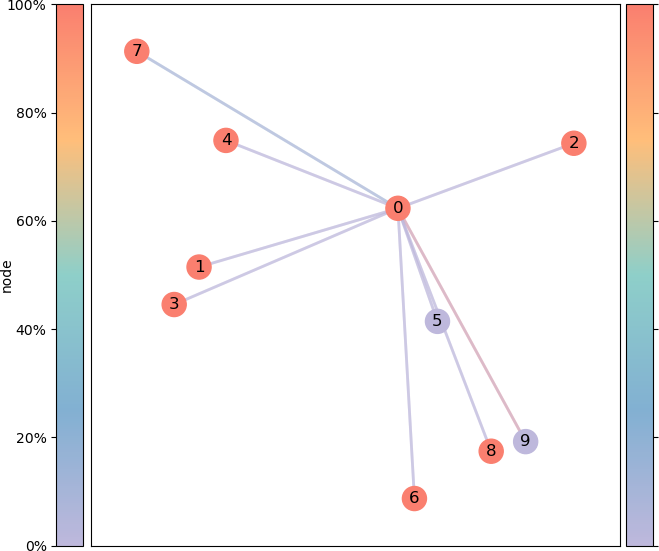
\includegraphics[width=0.75\linewidth]{figs/used_architecture.png}
    \caption{Used Architecture featuring Edge (Global Gateway), Fog (MDCs), and Cloud.}\label{fig:used_architecture}
\end{figure}


In Table~\ref{tab:node-specifications}, node specifications are listed, including Millions of Instructions Per Second (MIPS), the buffer size in GB, the up and down bandwidth from/to e0 (the global gateway) in GB and power coefficients in W. The network links range from 700 bps to 50,000 bps, forming a heterogeneous environment suitable for analyzing resource allocation and routing strategies under variable link constraints.


\begin{table*}[h!]
\centering

\resizebox{\columnwidth}{!}{%
\begin{tabular}{|l|c|c|c|c|c|c|c|c|l|}
\hline
\textbf{Node} & \textbf{Type} & \textbf{ID} & \textbf{MIPS} & \textbf{Buffer} & \textbf{Up BW} & \textbf{Down BW} & \textbf{Idle P} & \textbf{Exec P} & \textbf{Location} \\
\hline
e0 & Edge & 0 & 10 & 4 & -- & -- & 3 & 10 & Islamabad, PK \\ \hline
f0 & Fog & 1 & 110 & 16 & 2.5 & 1.7 & 30 & 150 & Multan, PK \\ \hline
f1 & Fog & 2 & 50 & 6 & 1 & 700 & 15 & 50 & Gilgit, PK \\ \hline
f2 & Fog & 3 & 95 & 12 & 2 & 1.5 & 25 & 120 & Karachi, PK \\ \hline
f3 & Fog & 4 & 85 & 10 & 1.5 & 1.2 & 20 & 100 & Lahore, PK \\ \hline
f4 & Fog & 5 & 75 & 8 & 1.2 & 1 & 20 & 100 & Peshawar, PK \\ \hline
c0 & Cloud & 6 & 500 & 51 & 3 & 3 & 300 & 1100 & Singapore \\ \hline
c1 & Cloud & 7 & 500 & 51 & 3 & 3 & 250 & 1000 & Belgium \\ \hline
\end{tabular}%
}
\caption{Detailed Specifications of Nodes}\label{tab:node-specifications}
\end{table*}


\subsection{Hyperparameters}

Since our modeling framework assigns zero latency and energy values to tasks that fail to be successfully offloaded, the primary optimization objective becomes the minimization of the \emph{task rejection rate}. This constraint is essential to prevent model degeneration, where the system could exploit the null assignment by deliberately rejecting tasks to artificially improve energy and latency performance metrics.

To further stabilize optimization, we adopt a hierarchical prioritization scheme that emphasizes latency over energy efficiency, as latency more directly impacts user experience and system responsiveness. This prioritization is reflected in the reward weight hierarchy:
\[
\lambda_0 \gg \lambda_1 > \lambda_2.
\]

Based on empirical evaluation of different configurations using a Multi-Layer Perceptron (MLP) architecture trained with Deep Q-Reinforcement Learning (DQL), we selected the following reward weight distribution:
\[
\textbf{Reward weights } (\lambda) = [1,\; 0.1,\; 0.05].
\]

Finally, to improve clarity and maintain consistency across training and evaluation, the energy consumption metric is reported in terms of power consumption throughout the experimental analysis.


\subsubsection{Model Configurations}

The complete hyperparameter specifications are detailed in Table~\ref{tab:model_specifications}. The MLP architectural parameters remain consistent across both Genetic Algorithm (GA)-based approaches and DQL implementations to ensure comparative validity.


\begin{table}[H]
\centering

\resizebox{\columnwidth}{!}{%
\begin{tabular}{|l|c|c|}
\hline
\textbf{Parameter} & \textbf{Transformer Model} & \textbf{MLP Model} \\ \hline
Hidden dimension ($d_{\text{model}}$) & 64 & 256 \\ \hline
Number of layers ($n_{\text{layers}}$) & 6 & 3 \\ \hline
Number of heads ($n_{\text{heads}}$) & 4 & - \\ \hline
Feed Forward Network ($d_{\text{ff}}$) & 256 & - \\ \hline
Dropout & 0.2 & 0 \\ \hline
Activation function & GELU & ReLU \\ \hline
Input features & \{cpu, bw, buffer\} & \{cpu, bw, buffer\} \\ \hline
\end{tabular}%
}
\caption{Model Specifications}\label{tab:model_specifications}
\end{table}

\subsubsection{Heuristic Baseline Methods}
We implement baseline heuristic approaches for comparative evaluation, namely, \emph{Random}, \emph{Round Robin (RR)} and \emph{Greedy}.

\paragraph{Random}
Random strategy, consist to randomly assign tasks to nodes uniformly at random, without consideration of current resource availability or node capabilities.

\paragraph{Round Robin}
RR is a straightforward load balancing technique where tasks are cyclically distributed among nodes, with each node receiving tasks in turn before cycling back to the first node. This ensures basic load balancing but ignores node heterogeneity such as CPU frequencies and buffer sizes, potentially causing inefficiencies under varied workloads. 

\paragraph{Greedy}
Greedy methods assign tasks based on immediate resource availability or specific cost metrics, such as selecting the node with the highest remaining CPU capacity. While easily implemented and computationally efficient, greedy strategies often forgo long-term, globally optimal decisions in favor of immediate local optima.



\subsection{Evaluation}

Table~\ref{tab:results_comparison} presents a detailed comparison of eight distinct offloading strategies, ranging from simple heuristic approaches to sophisticated machine learning-based methods. The results reveal significant performance variations across different algorithmic approaches.

\begin{table*}[htbp]
\centering

\begin{tabular}{lccc}
\textbf{Offloading Strategies} & \textbf{TTR (\%)} & \textbf{Latency (s)} & \textbf{Energy (W)} \\
\hline
Random 
 & 14.21
 & 20.89 
 & 238.3 \\
 
Round Robin 
 & 14.98
 & 18.36
 & 239.9 \\
\hline
\hline
 
Greedy 
 & 0.1889
 & 4.394
 & 338.7 \\

\hline
 
MLP 
 & 0.1111
 & 4.332
 & 349.0 \\
 
NOTE 
 & \textbf{0.0000} 
 & 4.150
 & 337.6 \\
 
T-NOTE 
 & \textbf{0.0000} 
 & \textbf{3.663} 
 & \textbf{317.0} \\

\end{tabular}

\caption{Comparison of Offloading Strategies with Task Throw Rate (TTR), Latency (\(L\)), and Energy (\(E\)) on Pakistan test set.
Best results are in \textbf{bold}.}
\label{tab:results_comparison}
\end{table*}

Random and Round Robin exhibit high Task Throw Rates (TTR) exceeding 14\% and latency over 18 seconds. This is due to their simplistic task assignment mechanisms, which do not account for the varying resource capacities of nodes but rather distribute tasks evenly, favoring energy efficiency as more fog nodes are utilized~\ref{subsec:random}. In contrast, the Greedy approach significantly reduces TTR to 0.1889\% and latency to 4.3936 seconds by prioritizing nodes with the highest available CPU resources~\ref{subsec:greedy-baseline}. However, this comes at the cost of increased energy consumption (338.6652 W) due to the overutilization of high-capacity nodes. Since this paper focuses primarily on minimizing TTR, the Greedy method's performance is taken as the baseline.

The DQL-based approaches demonstrate substantial improvements over the Greedy baseline, with progressively refined architectures yielding incrementally better performance. The MLP strategy achieves a TTR of 0.1111\%, representing a 41.2\% reduction compared to Greedy, while simultaneously reducing latency to 4.3315 seconds (a 1.4\% improvement). However, this comes at the expense of higher energy consumption (348.9158 W, 3.0\% increase over Greedy), suggesting that the MLP's learned offloading policy favors reliability and speed over energy efficiency. The transformer-based NOTE architecture further advances performance by eliminating task failures entirely (0.0000\% TTR) and reducing latency to 4.1504 seconds (5.5\% improvement over Greedy), while maintaining comparable energy consumption (337.5961 W). This improvement stems from the transformer encoder's ability to capture complex relationships between node observations through self-attention mechanisms. Building upon this foundation, T-NOTE extends the architecture by incorporating task-level observations alongside node characteristics, enabling the model to make more contextually aware offloading decisions. This extension yields the best overall performance across all metrics: maintaining zero task failures while achieving the lowest latency (3.6626 seconds, 16.6\% improvement over Greedy) and the most efficient energy consumption (317.0230 W, 6.4\% reduction compared to Greedy), demonstrating that task-aware attention mechanisms enable superior resource allocation strategies.


\subsection{MLP-Based DQL}\label{subsec:mlp_perf}

The MLP-based DQL approach utilizes a feed-forward neural network to estimate Q-values for each node based on the current state of the system, which includes CPU availability, buffer size, and link bandwidth. 

\paragraph{Robustness and Performance}

The MLP-based DQL approach exhibits sensitivity to hyperparameter configurations, particularly the learning rate and reward weights. While it can achieve performance improvements over heuristic baselines, its convergence behavior is less stable compared to Transformer-based methods. The MLP's limited capacity may contribute to this instability, as it relies on fixed-size input vectors.


\paragraph{Convergence Analysis}

Figure~\ref{fig:mlp-score-plot} illustrates the convergence behavior of the MLP-based DQL model over training epochs. The best model is picked based on the highest average score, which combines TTR, L and E metrics with reward weights, at the 9th epoch. 

\begin{figure}[H]
    \centering
    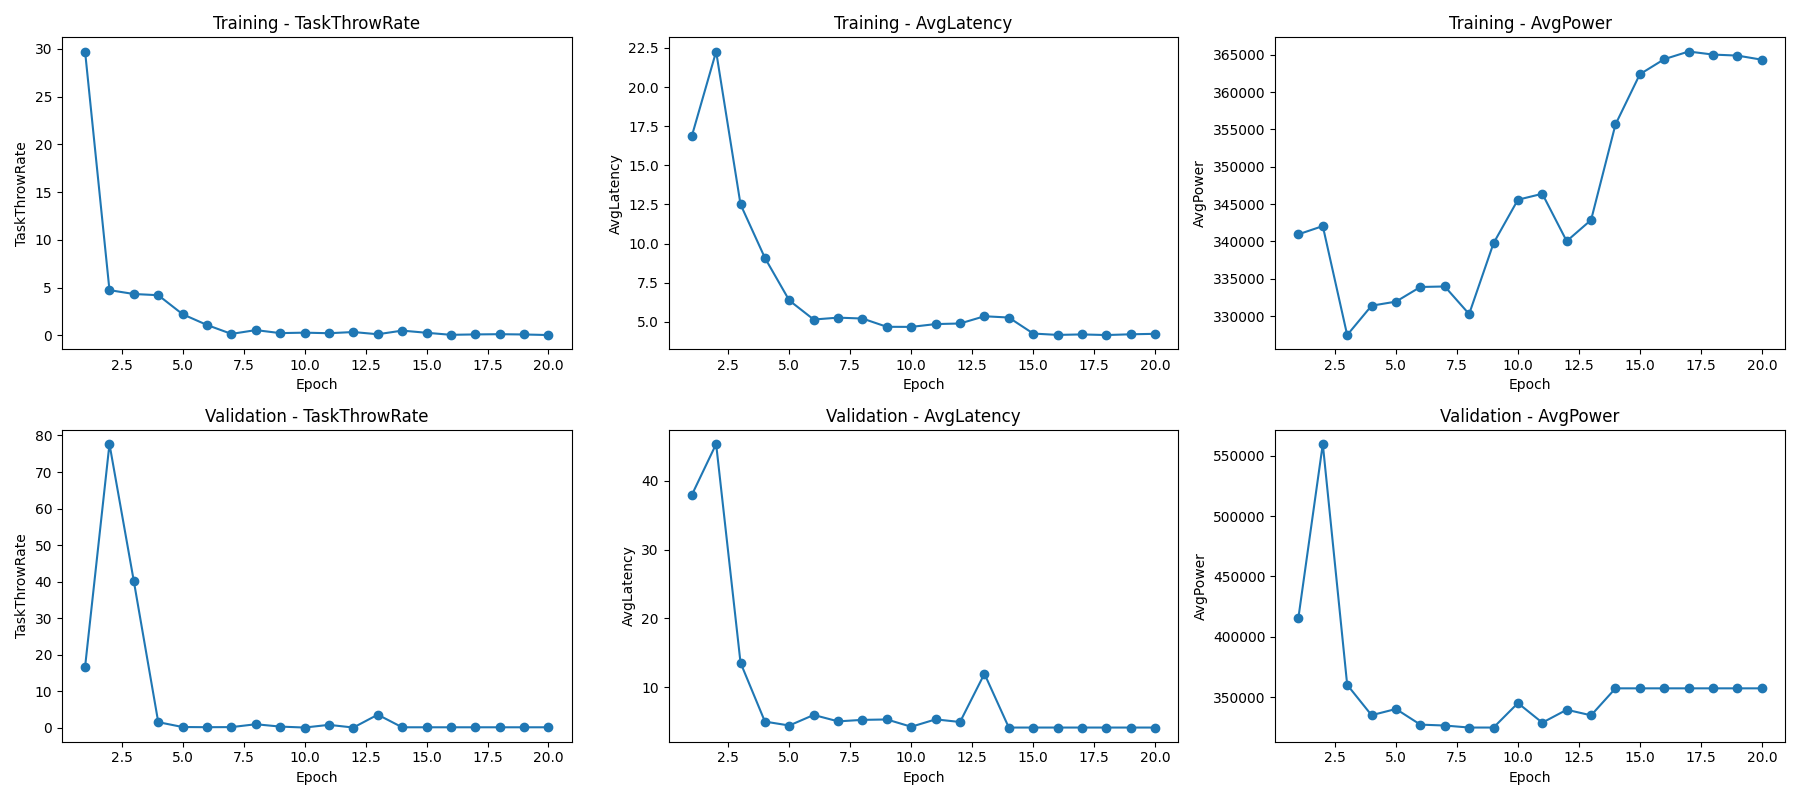
\includegraphics[width=1\linewidth]{figs/MLP/score_plot.png}
    \caption{Convergence and Scores for MLP-Based DQL}\label{fig:mlp-score-plot}
\end{figure}




\subsection{Transformer-Based DQL}\label{subsec:transformer_perf}

Transformer architectures, such as NOTE and T-NOTE, were also evaluated under a DQL paradigm. Although these models have far more parameters (e.g., around 350k, which is roughly 50 times more than the MLP), they have demonstrated superior performance in practice. 

\paragraph{Robustness and Performance}
Despite their complexity, the self-attention mechanisms in NOTE and T-NOTE appear more robust to hyperparameter variations, converging to superior solutions that surpass the MLP-based approaches. This finding aligns with~\cite{gholipour_tpto_2023}, suggesting that Transformers can effectively capture nuanced interactions between tasks and nodes. 



\subsubsection{NOTE}
NOTE encodes only node-level features (CPU, buffer, bandwidth), aggregated over tasks. As illustrated in Figure~\ref{fig:NOTE-score-plot}, the learning process initially exhibits some fluctuation but gradually settles into a stable solution. This convergence highlights the capability of self-attention to capture and refine relationships among multiple nodes. Although small oscillations persist, the overall trend consistently improves latency and task throughput rates.

\begin{figure}[H]
    \centering
    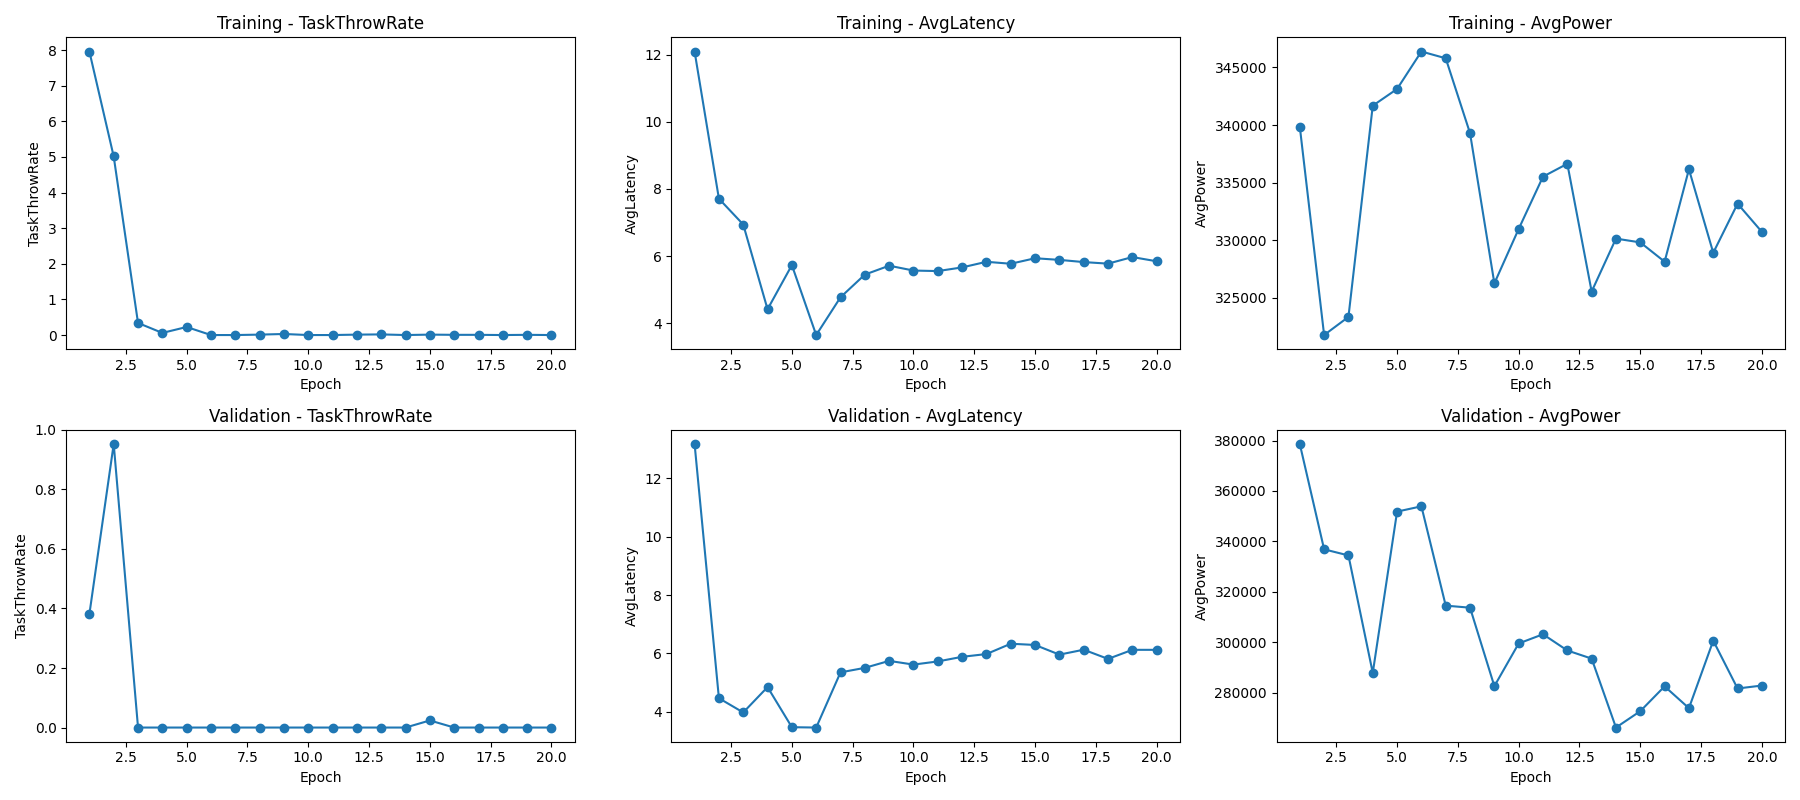
\includegraphics[width=1\linewidth]{figs/NOTE/score_plot.png}
    \caption{Convergence and Scores for NOTE-Based DQL}
    \label{fig:NOTE-score-plot}
\end{figure}

\subsubsection{T-NOTE}
T-NOTE augments NOTE by including task attributes (size, deadline, CPU-cycle requirements). These additional features allow the model to make more informed offloading decisions, resulting in faster convergence and often superior performance in terms of latency and success rate. Figure~\ref{fig:T-NOTE-score-plot} shows that T-NOTE reaches an optimal solution around the third epoch, but then experiences slight performance degradation as training continues. This fluctuation may occur because:
\begin{itemize}
    \item The task-specific embeddings introduce additional complexity, potentially causing the network to overfit or oscillate when new tasks arrive.
    \item DQL’s state representation depends on real-time task information, not just node-level resources.
\end{itemize}
Despite these variations, T-NOTE still surpasses NOTE in both speed of convergence and final performance, demonstrating the value of incorporating task-aware embeddings.

\begin{figure}[H]
    \centering
    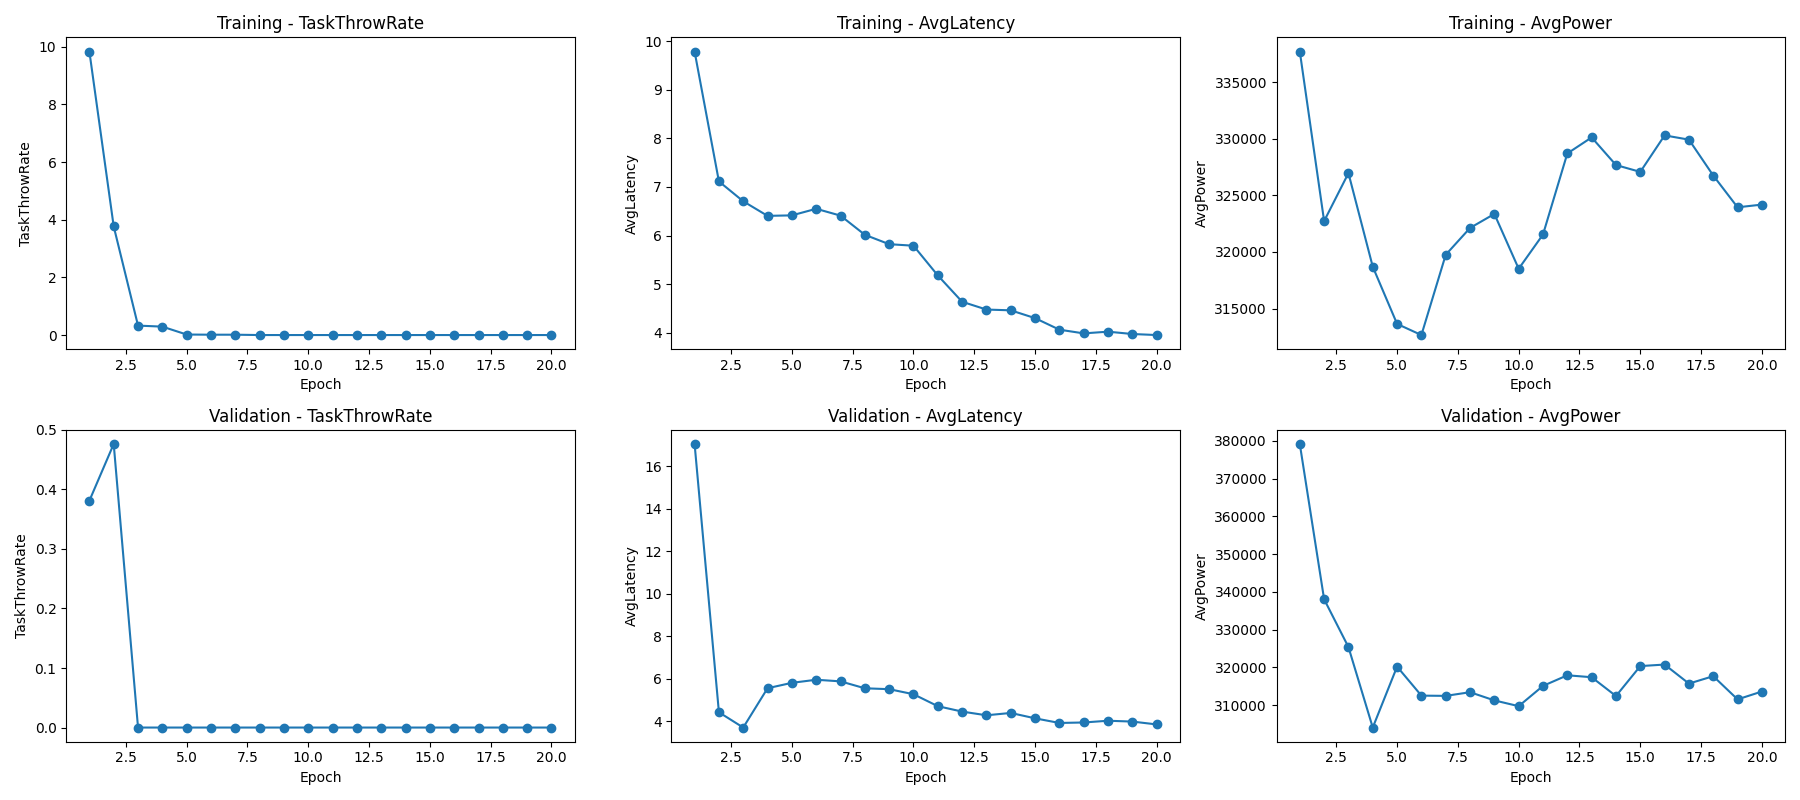
\includegraphics[width=1\linewidth]{figs/T-NOTE/score_plot.png}
    \caption{Convergence and Scores for T-NOTE-Based DQL}
    \label{fig:T-NOTE-score-plot}
\end{figure}



\subsection{Offloading Analysis}\label{subsec:offloading-analysis}

This section presents a comprehensive analysis of the offloading strategies employed by different approaches, examining their performance characteristics, resource utilization patterns, and trade-offs. The analysis is structured to provide insights into how each method addresses the fundamental challenges of task allocation in hierarchical edge-fog-cloud computing environments.

A comparative evaluation of offloading policies reveals that \emph{Transformer-based DQL} demonstrates superior robustness by achieving an optimal balance between latency minimization and TTR compared to alternative approaches. While multi-objective GA methods provide a diverse set of Pareto-optimal solutions enabling flexible trade-off selection, MLP-based DQL maintains computational efficiency as its primary advantage. The following subsections provide detailed analysis of node utilization patterns, performance metrics, and the underlying decision-making characteristics of selected methodologies.

\subsubsection{Random}
\label{subsec:random}

The Random offloading strategy serves as a baseline for evaluating the effectiveness of more sophisticated task allocation policies in hierarchical edge-fog-cloud environments. By randomly assigning tasks to available nodes, this approach lacks any awareness of the underlying resource capabilities, often leading to inefficient resource utilization and increased latency.

\begin{figure}[H]
    \centering
    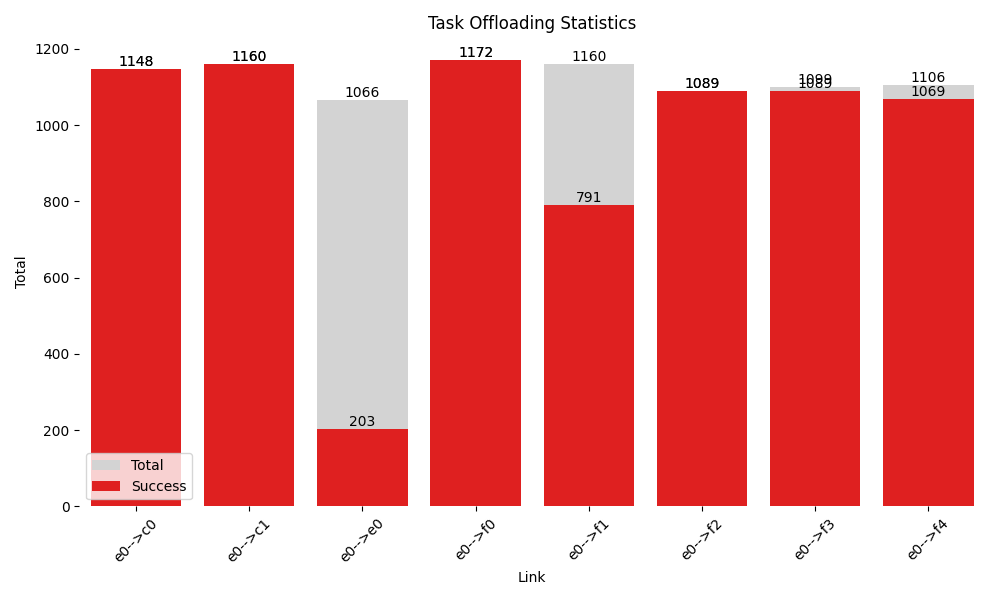
\includegraphics[width=0.5\linewidth]{figs/Random/task_offloading_statistics.png}
    \caption{Task offloading distribution across node types for the Random baseline}
    \label{fig:random-task-offloading-stats}
\end{figure}

\begin{figure}[H]
    \centering
    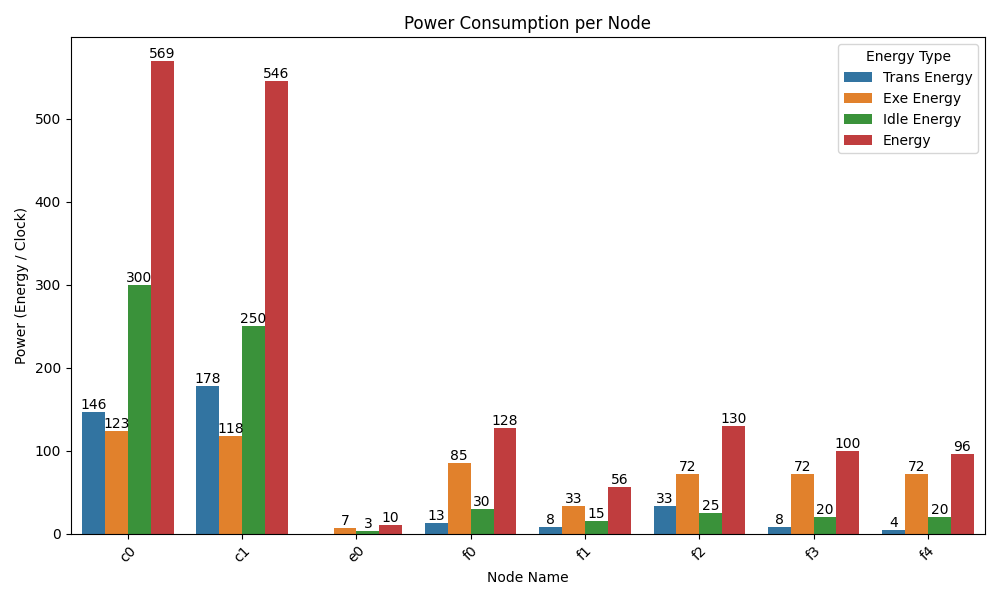
\includegraphics[width=0.5\linewidth]{figs/Random/power_consumption_per_node.png}
    \caption{Power consumption per node for the Random baseline}
    \label{fig:random-power-consumption}
\end{figure}



\subsubsection{Greedy (baseline)}
\label{subsec:greedy-baseline}

The Greedy offloading strategy serves as a fundamental baseline for evaluating the effectiveness of more sophisticated task allocation policies in hierarchical edge-fog-cloud environments. The Greedy method's simplicity enables rapid decision-making but often leads to suboptimal global performance due to its myopic nature. 


\begin{figure}[H]
    \centering
    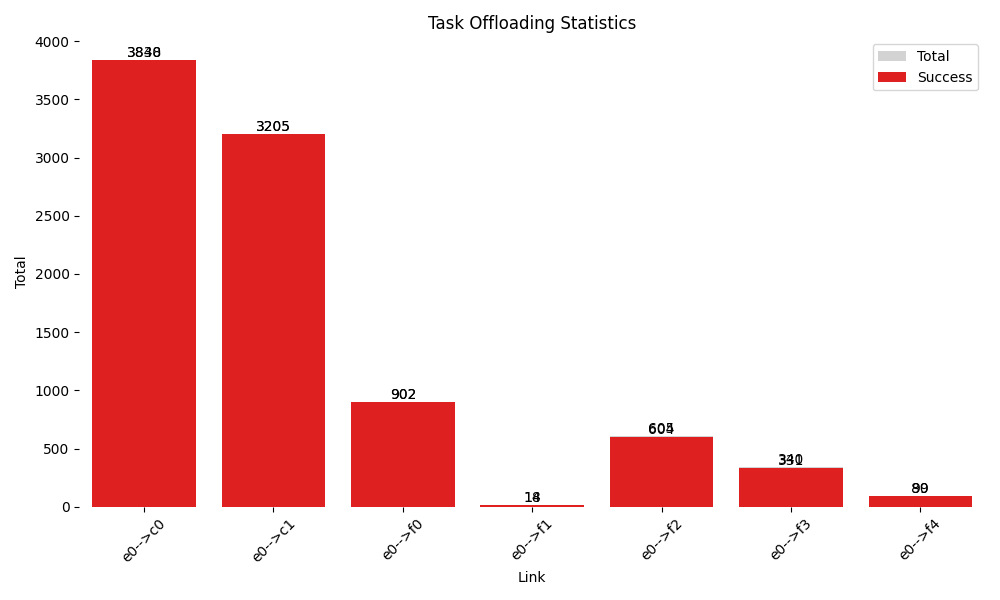
\includegraphics[width=0.5\linewidth]{figs/Greedy/task_offloading_statistics.png}
    \caption{Task offloading distribution across node types for the Greedy baseline}
    \label{fig:greedy-task-offloading-stats}
\end{figure}

Figure~\ref{fig:greedy-task-offloading-stats} illustrates the distribution of task assignments across edge, fog, and cloud nodes under the Greedy policy. The results indicate a strong preference for offloading to nodes with the higher CPU frequency, often resulting in a disproportionate allocation to cloud nodes, making these nodes more asked for CPU resources as illustrated in Figure~\ref{fig:greedy-cpu-freq}.



\begin{figure}[H]
    \centering
    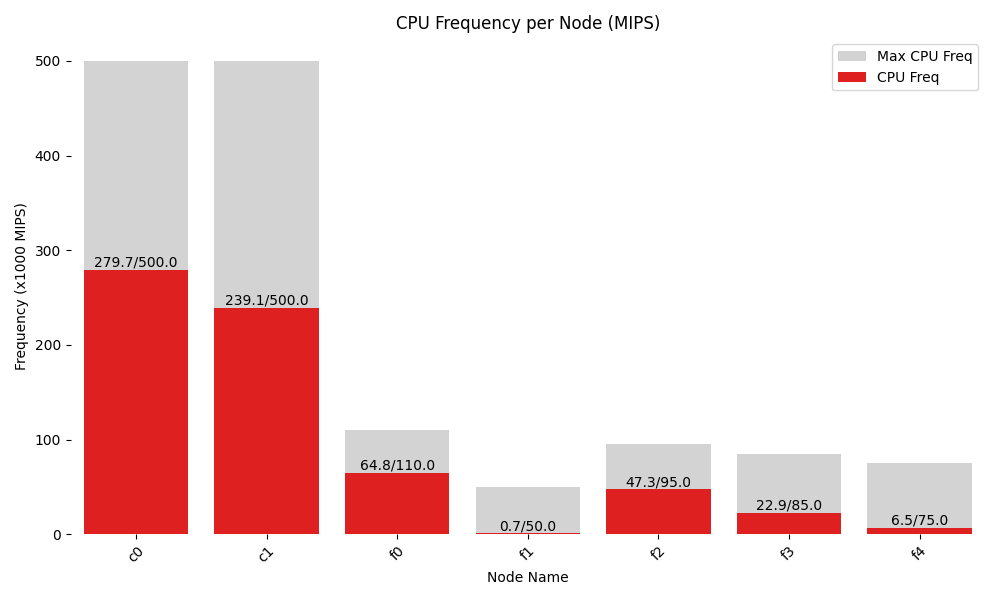
\includegraphics[width=0.5\linewidth]{figs/Greedy/cpu_frequency_per_node.png}
    \caption{Average CPU frequency utilization per node for the Greedy baseline.}
    \label{fig:greedy-cpu-freq}
\end{figure}


The average communication latency per network link, depicted in Figure~\ref{fig:greedy-avg-latency}, demonstrates that the Greedy approach achieves moderate latency performance under typical load conditions. 

\begin{figure}[H]
    \centering
    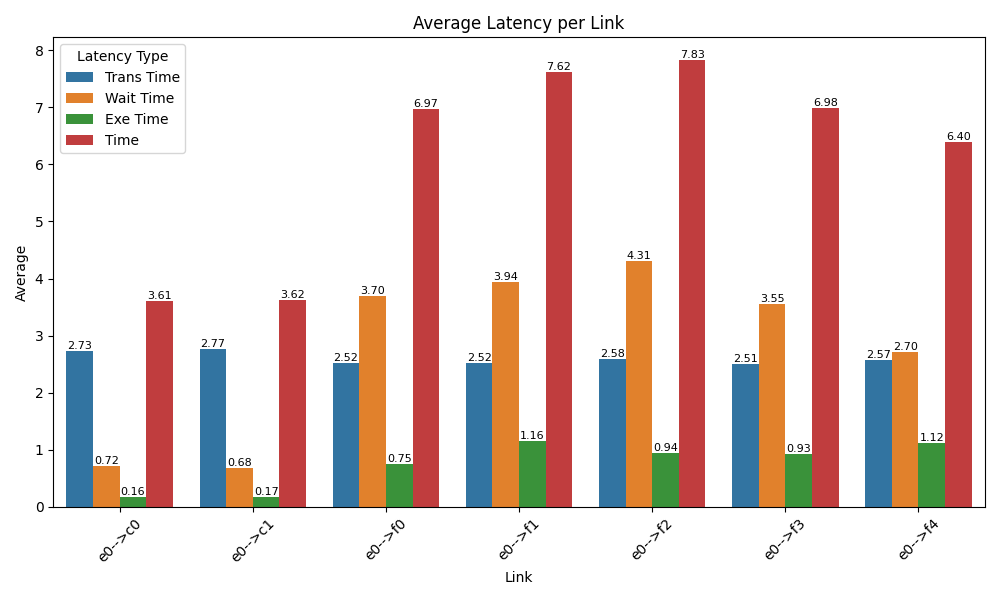
\includegraphics[width=0.5\linewidth]{figs/Greedy/avg_latency_per_link.png}
    \caption{Average communication latency per network link for the Greedy baseline.}
    \label{fig:greedy-avg-latency}
\end{figure}


Figures~\ref{fig:greedy-power-consumption} present the power consumption across different nodes. The Greedy policy's tendency to overload cloud nodes leads to localized energy hotspots and increased power draw at the cloud tier. In contrast, fog nodes remain underutilized except during peak demand, resulting in an uneven distribution of energy consumption throughout the system.

\begin{figure}[H]
    \centering
    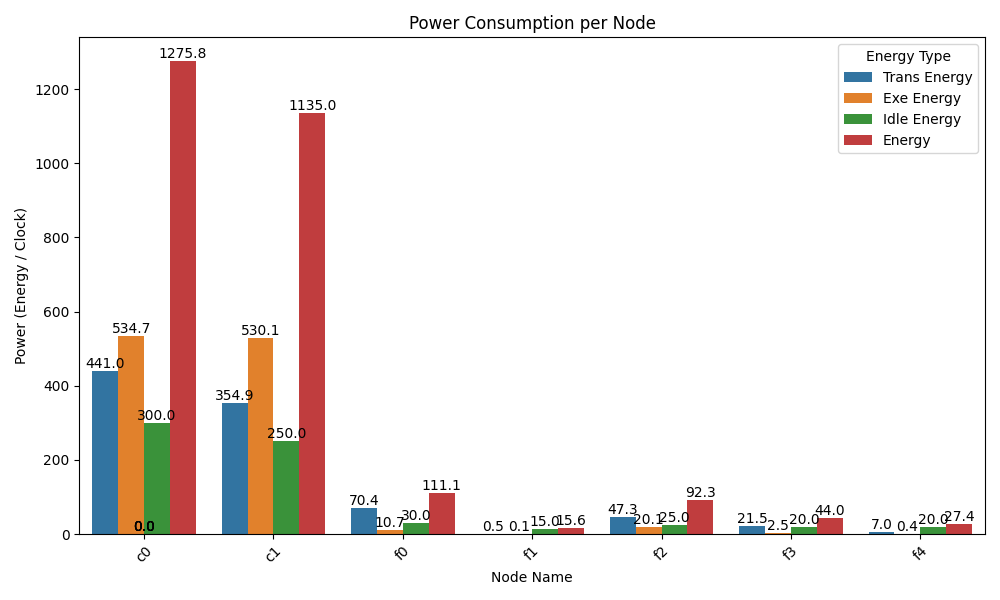
\includegraphics[width=0.5\linewidth]{figs/Greedy/power_consumption_per_node.png}
    \caption{Power consumption distribution across different node types for the Greedy baseline.}
    \label{fig:greedy-power-consumption}
\end{figure}


\subsubsection{MLP-Based DQL Performance Analysis}\label{subsubsec:mlp-DQL-analysis}

The MLP-based approach, whether evolved through genetic algorithms or trained via deep Q-learning, demonstrates convergence to similar offloading patterns in the final policy. For comprehensive analysis, this study focuses on the DQL variant of the MLP implementation, as the solution founded for DQL is really near than the GA-based multi-objective that minimize the reward weights $(\lambda)$.

As illustrated in Figure~\ref{fig:mlp-task-offloading-stats}, the MLP-based policy exhibits an aggressive cloud-centric offloading strategy. This approach prioritizes cloud node utilization to minimize both task throw rate (TTR) and processing latency, directly reflecting the optimization objective defined by the high weighting factors $\lambda_0$ (failure penalty) and $\lambda_1$ (latency penalty) in the reward function. The policy demonstrates a clear preference for leveraging the superior computational resources available in cloud nodes, which possess higher processing capabilities and more stable connectivity compared to edge and fog alternatives.

\begin{figure}[H]
    \centering
    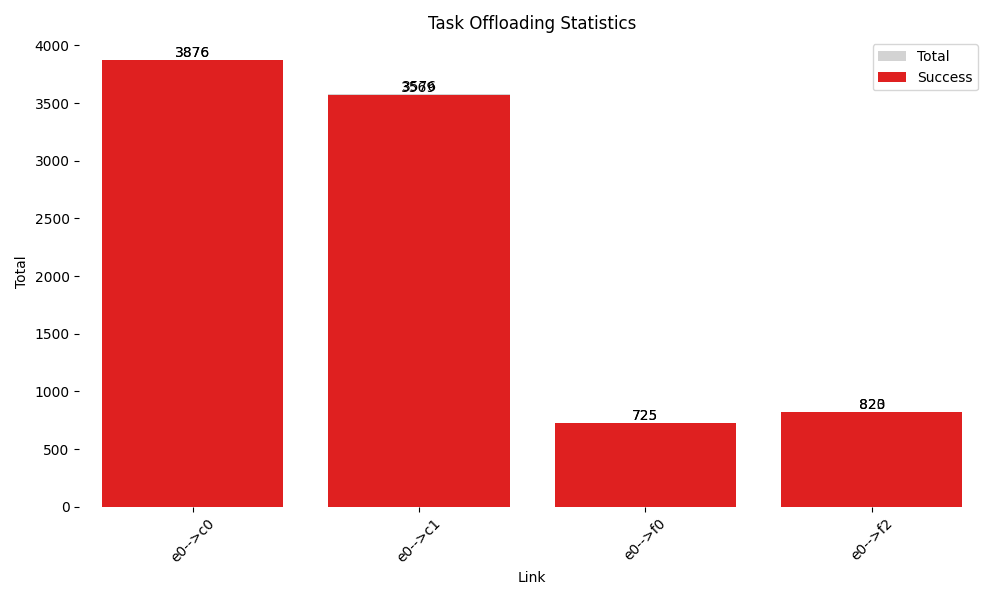
\includegraphics[width=0.5\linewidth]{figs/MLP/task_offloading_statistics.png}
    \caption{Task offloading distribution across node types for MLP-based DQL, showing the proportion of tasks allocated to edge, fog, and cloud nodes}
    \label{fig:mlp-task-offloading-stats}
\end{figure}

However, this strategy results in significant underutilization of fog devices, as any tasks are offloaded to the fog, which represents an intermediate tier of computational resources that could potentially provide a more balanced trade-off between performance and energy efficiency. The heavy reliance on cloud computing infrastructure leads to a concentration of energy consumption at the cloud level, as depicted in the subsequent power consumption analysis.

\begin{figure}[H]
    \centering
    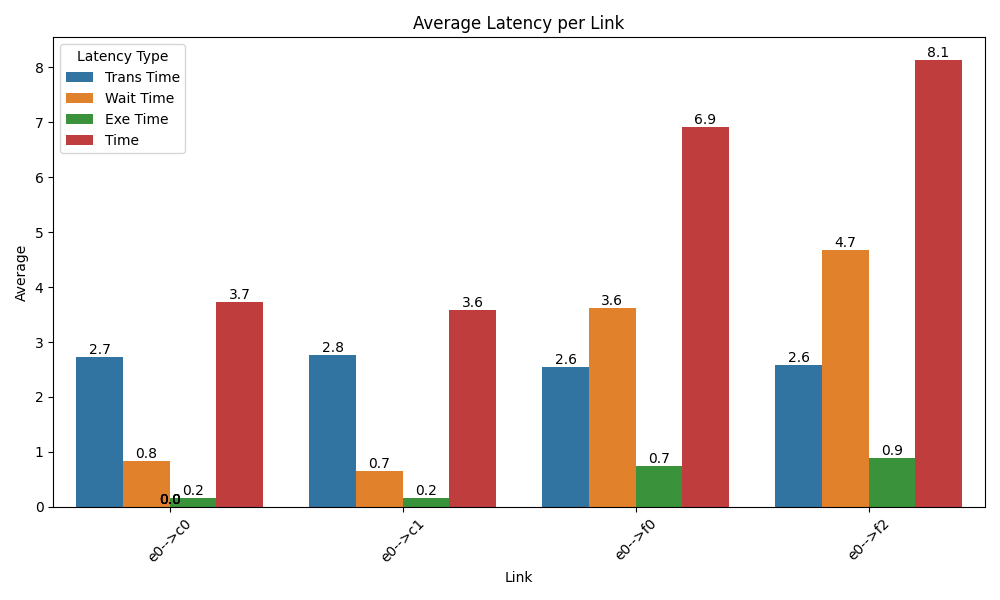
\includegraphics[width=0.5\linewidth]{figs/MLP/avg_latency_per_link.png}
    \caption{Average communication latency per network link for MLP-based DQL}
    \label{fig:mlp-avg-latency}
\end{figure}

\begin{figure}[H]
    \centering
    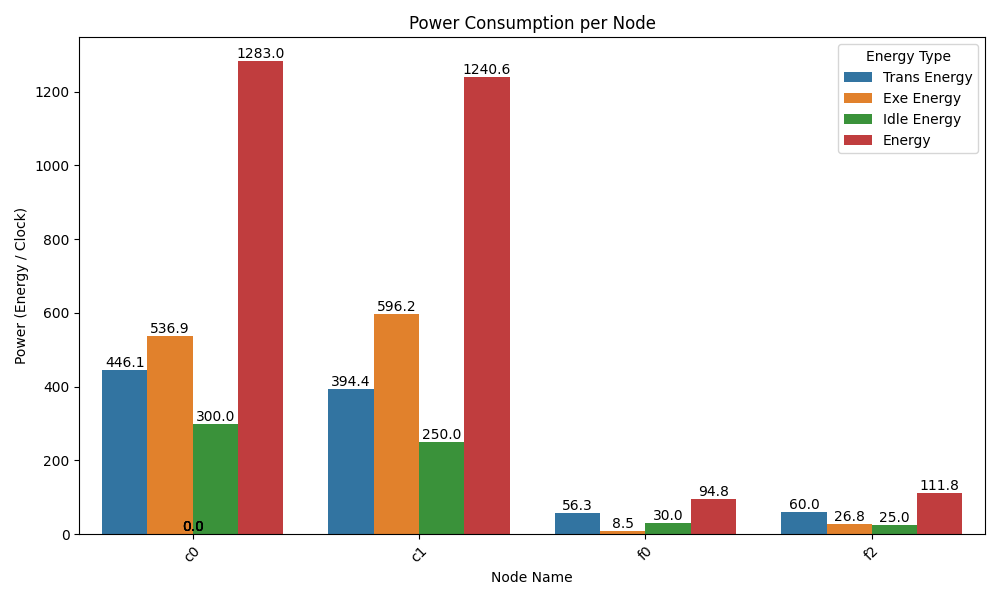
\includegraphics[width=0.5\linewidth]{figs/MLP/power_consumption_per_node.png}
    \caption{Power consumption distribution across different node types for MLP-based DQL}
    \label{fig:mlp-power-consumption}
\end{figure}

The performance characteristics shown in Figures~\ref{fig:mlp-avg-latency} and~\ref{fig:mlp-power-consumption} confirm the cloud-centric strategy's effectiveness in achieving low latency objectives while simultaneously revealing its limitations in terms of energy distribution. The concentration of task processing at cloud nodes results in minimal communication and processing latency but creates a substantial energy burden on cloud infrastructure. This trade-off reflects the single-objective optimization focus inherent in the DQL approach, where the primary goal is to maximize a unified reward function rather than explicitly balancing multiple competing objectives.


\subsubsection{Transformer-Based DQL (T-NOTE)}\label{subsubsec:T-NOTE-analysis}

The T-NOTE architecture represents a significant advancement over traditional MLP-based approaches by incorporating explicit attention mechanisms for task attribute processing. While both NOTE and T-NOTE variants demonstrate improvements over MLP-based solutions, T-NOTE consistently outperforms NOTE due to its enhanced capability to model task-specific characteristics and their relationships to optimal node selection.

\begin{figure}[H]
    \centering
    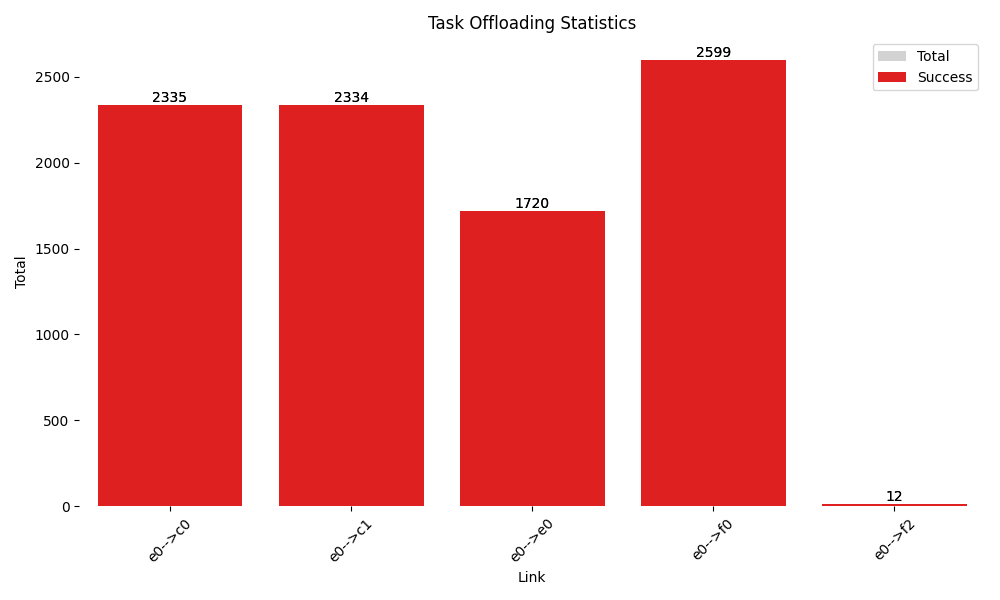
\includegraphics[width=0.5\linewidth]{figs/T-NOTE/task_offloading_statistics.png}
    \caption{Task offloading distribution for T-NOTE}
    \label{fig:T-NOTE-offloading-stats}
\end{figure}

Figure~\ref{fig:T-NOTE-offloading-stats} reveals that T-NOTE maintains a preference for cloud nodes while demonstrating more sophisticated resource allocation strategies. The approach judiciously employs fog resources when cloud queues experience congestion or when specific tasks require lower-latency local processing. This adaptive behavior stems from the Transformer architecture's ability to capture complex relationships between task characteristics, network conditions, and node capabilities through its attention mechanism.

The balanced allocation strategy becomes more apparent when examining the latency characteristics across different network links. Unlike the MLP approach, T-NOTE occasionally utilizes edge nodes for specific use cases, particularly for small computational tasks or time-sensitive operations where local processing provides advantages despite limited computational resources.

\begin{figure}[H]
    \centering
    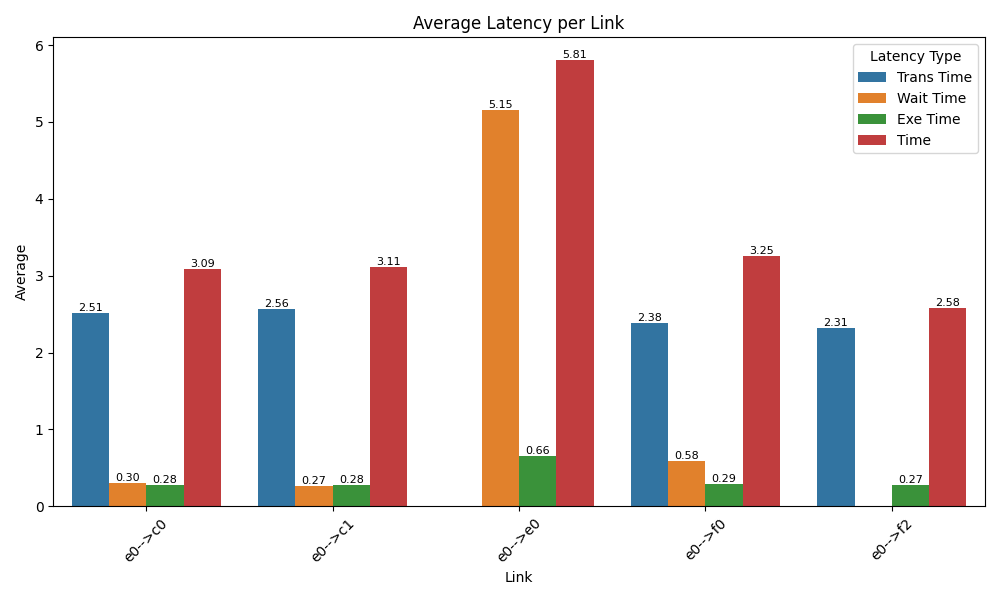
\includegraphics[width=0.5\linewidth]{figs/T-NOTE/avg_latency_per_link.png}
    \caption{Average latency per network link for T-NOTE}
    \label{fig:T-NOTE-avg-latency}
\end{figure}

\begin{figure}[H]
    \centering
    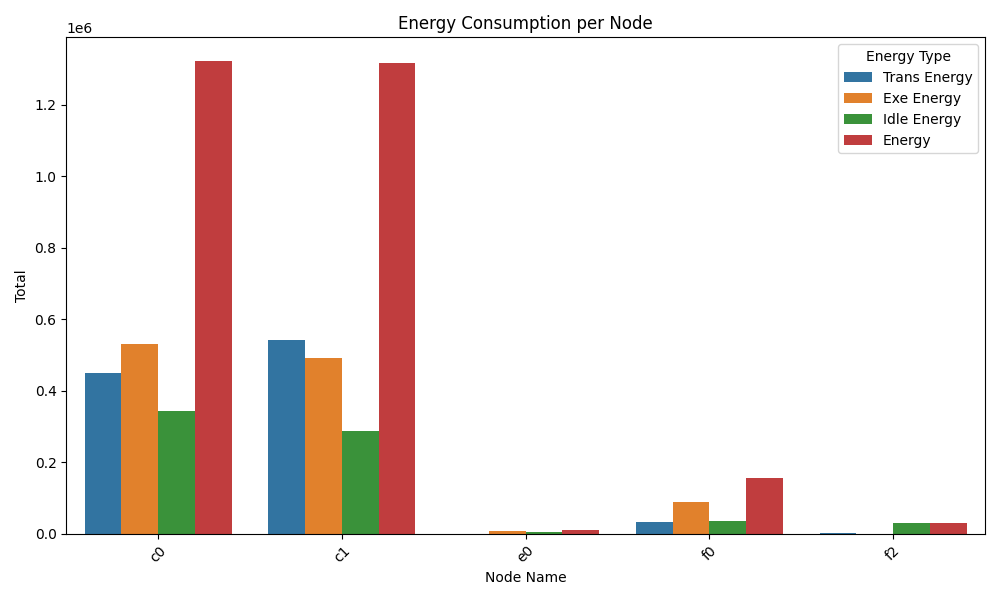
\includegraphics[width=0.5\linewidth]{figs/T-NOTE/energy_consumption_per_node.png}
    \caption{Energy consumption distribution for T-NOTE}
    \label{fig:T-NOTE-energy-consumption}
\end{figure}

\begin{figure}[H]
    \centering
    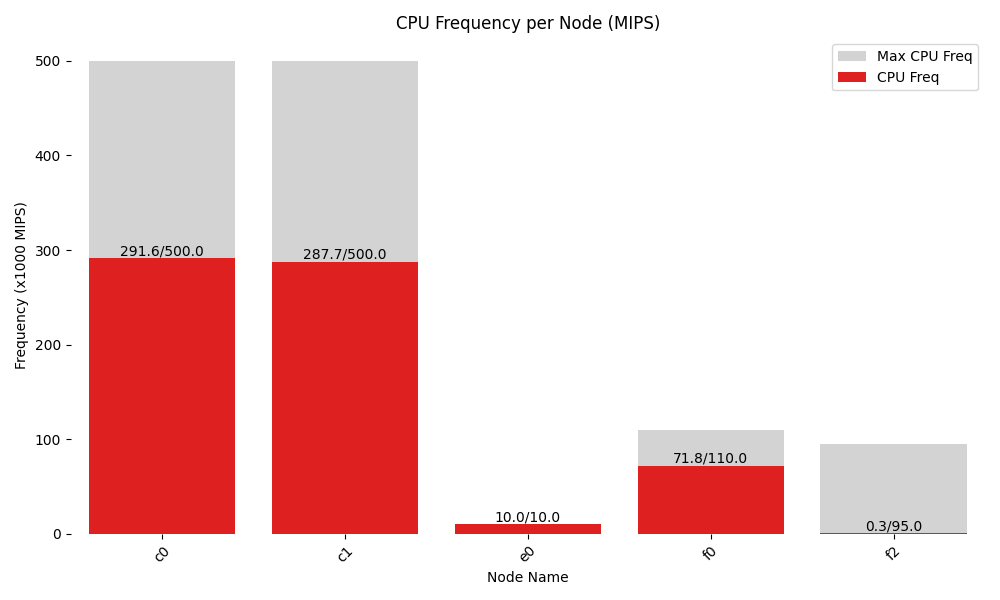
\includegraphics[width=0.5\linewidth]{figs/T-NOTE/cpu_frequency_per_node.png}
    \caption{CPU frequency utilization per node type for T-NOTE}
    \label{fig:T-NOTE-cpu-frequency}
\end{figure}

The energy consumption and CPU utilization patterns shown in Figures~\ref{fig:T-NOTE-energy-consumption} and \ref{fig:T-NOTE-cpu-frequency} illustrate that cloud nodes continue to dominate in both power usage and computational utilization. This dominance aligns with the high resource availability at cloud level and the reward function's emphasis on minimizing task failures and processing latency. However, the partial utilization of fog nodes represents a strategic improvement over the MLP approach, as it helps mitigate congestion at the cloud level while maintaining overall system performance.

The T-NOTE's adaptive decision-making capability enables it to recognize scenarios where distributed processing across multiple node types provides superior outcomes compared to pure cloud-centric strategies. This flexibility becomes particularly valuable under varying network conditions and diverse task requirements, demonstrating the architecture's potential for real-world deployment scenarios where computational demands and network characteristics exhibit significant temporal and spatial variation.

\subsection{Energy Consideration}\label{sec:energy_consideration}

To highlight the performance of the proposed DRL-based approaches with respect to energy consumption, we compare T-NOTE, our best model, with the heuristic baselines, Random and Round Robin, as shown in Table~\ref{tab:energy_comparison}. By appropriately adjusting the reward weights to prioritize energy efficiency, T-NOTE achieves 40 times lower TTR and 3.5 times lower latency than the heuristic baselines, while maintaining comparable energy consumption. This demonstrates that T-NOTE can be adapted to different optimization objectives through reward weight tuning, highlighting the effectiveness and flexibility of the proposed DRL-based approach in optimizing task offloading across hierarchical edge-fog-cloud environments.

\begin{table*}[htbp]
\centering

\begin{tabular}{lccc}
\textbf{Offloading Strategies} & \textbf{TTR (\%)} & \textbf{Latency (s)} & \textbf{Energy (W)} \\
\hline
Random 
 & 14.21
 & 20.89
 & 238.3 \\
 
Round Robin 
 & 14.98
 & 18.36
 & 239.9 \\
 
T-NOTE 
 & \textbf{0.3556} 
 & \textbf{5.976} 
 & \textbf{238.0} \\

\end{tabular}

\caption{Performance comparison of T-NOTE with energy-optimized reward weights against heuristic baselines on Pakistan test set. Best results are in \textbf{bold}.}
\label{tab:energy_comparison}
\end{table*}



\subsection{GA-based Results and Comparison}\label{subsec:ga_vs_DQL}

Both the GA-based (NSGA II and NPGA) and DQL methods can train a MLP with 6,664 trainable parameters, using the same input features (CPU, buffer, and bandwidth). However, each approach yields distinct convergence properties and solution spaces.

\subsubsection{Convergence Behavior}
\paragraph{GA-based}
The GA-based approach is more sensitive to initial population generation, and convergence behaviors can vary widely with different random seeds. As shown in Figure~\ref{fig:nsga2-mlp-training-epoch} for NSGA II, wich is almost similar to NPGA, training often exhibits fluctuations when searching for Pareto-optimal solutions, especially in the early stages of evolution. Although the algorithm eventually discovers high-quality solutions, it may require many generations (e.g., 100 generations with 40 individuals each) to achieve consistency.

\begin{figure}[H]
    \centering
    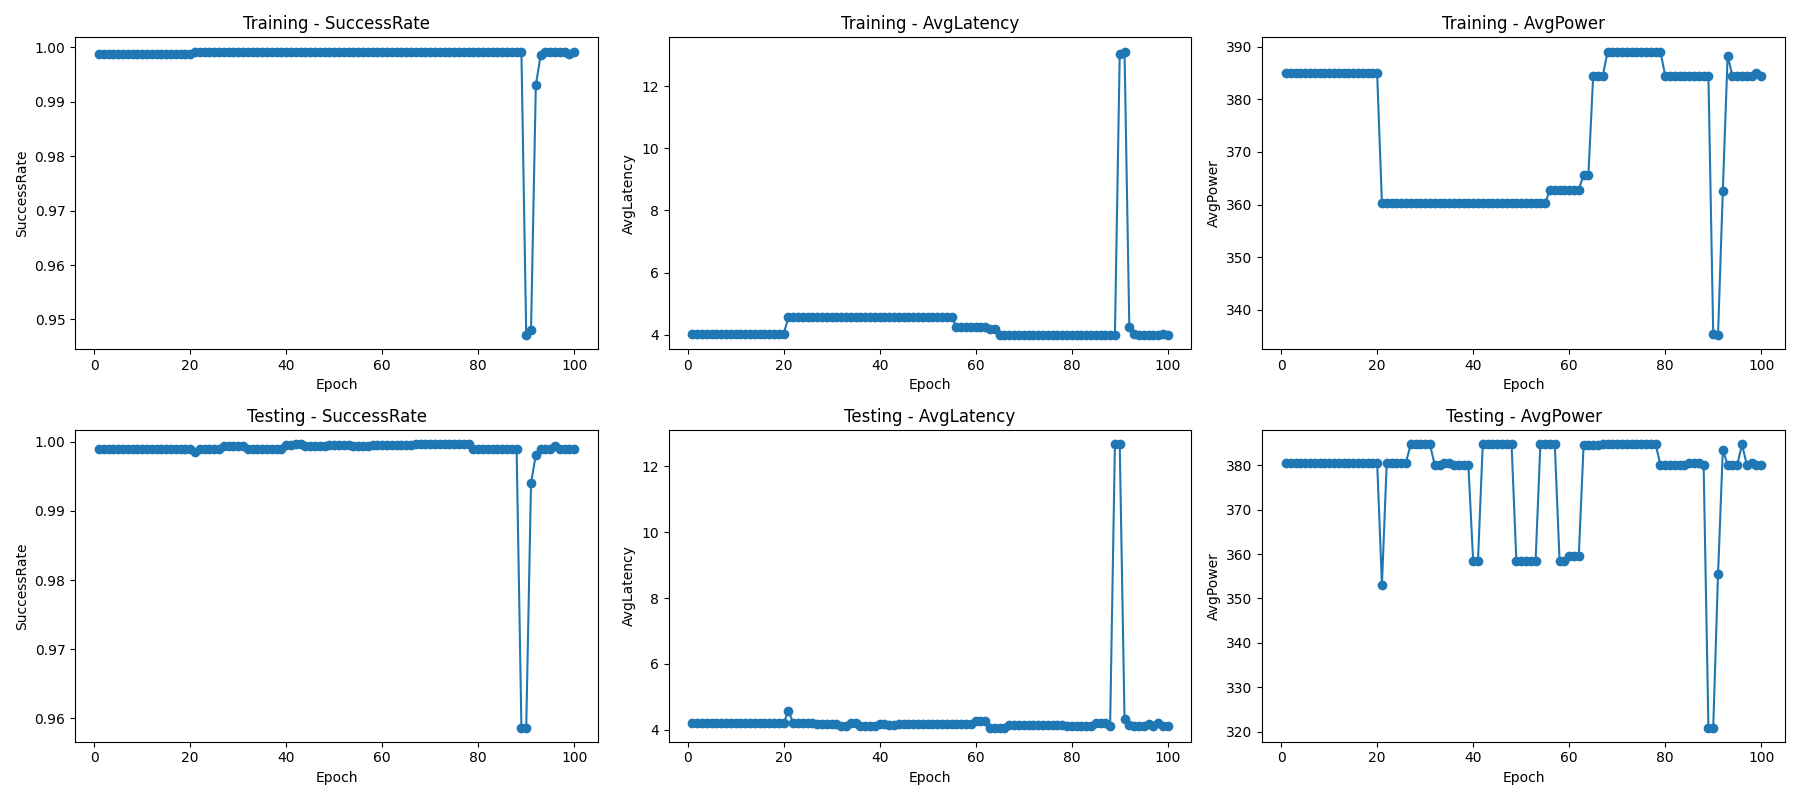
\includegraphics[width=0.95\linewidth]{figs/nsga2_mlp_training_epoch.png}
    \caption{Training Convergence for MLP with NSGA2 for the best individual, selected according to \(\lambda_0 \gg \lambda_1 \gg \lambda_2\).}  
    \label{fig:nsga2-mlp-training-epoch}  
\end{figure}



\paragraph{Performance}

\begin{table*}[htbp]
\centering


\begin{tabular}{lccc}

\textbf{Offloading Strategies} & \textbf{TTR (\%)} & \textbf{Latency (s)} & \textbf{Energy (W)} \\

\hline

NSGA2 + MLP 
 & \underline{0.07} 
 & 4.16
 & 385 \\
 
NPGA + MLP 
 & 0.14 
 & 4.24 
 & 380 \\
 
DQL + MLP 
 & \underline{0.07} 
 & 4.16 
 & 385 \\
 


\end{tabular}

\caption{Comparison of MLP with DQL, NPGA, and NSGA2 on Pakistan test set.}\label{tab:mlp_comparison}
\end{table*}


\paragraph{Trade-Off in Efficiency}
A key advantage of DQL is the reduced computational burden—only one model is trained and updated across epochs (e.g., 10–20 epochs), compared to GA approaches that must evaluate a large population (e.g., 40 individuals) for multiple generations (e.g., 100). Hence, GA methods generally consume more time hours despite their ability to track multiple objectives.

\subsubsection{Solution Space and Pareto Frontiers}
Although DQL is effectively treating the problem as a single-objective function (via the weighted sum of different metrics in the reward), multi-objective GA methods (e.g., NSGA2, NPGA) discover a \emph{set} of Pareto-optimal solutions. This advantage is illustrated in Figures~\ref{fig:nsga2-pareto-frontiers} and~\ref{fig:npga-pareto-frontiers}, where multiple configurations of (latency, energy, throw rate) emerge along the final Pareto front. Practitioners can then choose the solution that best fits their operational needs (e.g., emphasizing latency more strongly or focusing on energy savings).

DQL produces a single high-performing policy, which in practice falls somewhere within or near the Pareto front discovered by GA. Experimental results indicate that the DQL policy is generally comparable to those in the GA’s Pareto set. However, users requiring fine-grained trade-offs among metrics may prefer GA-based multi-objective solutions.

\begin{figure}[H]
    \centering
    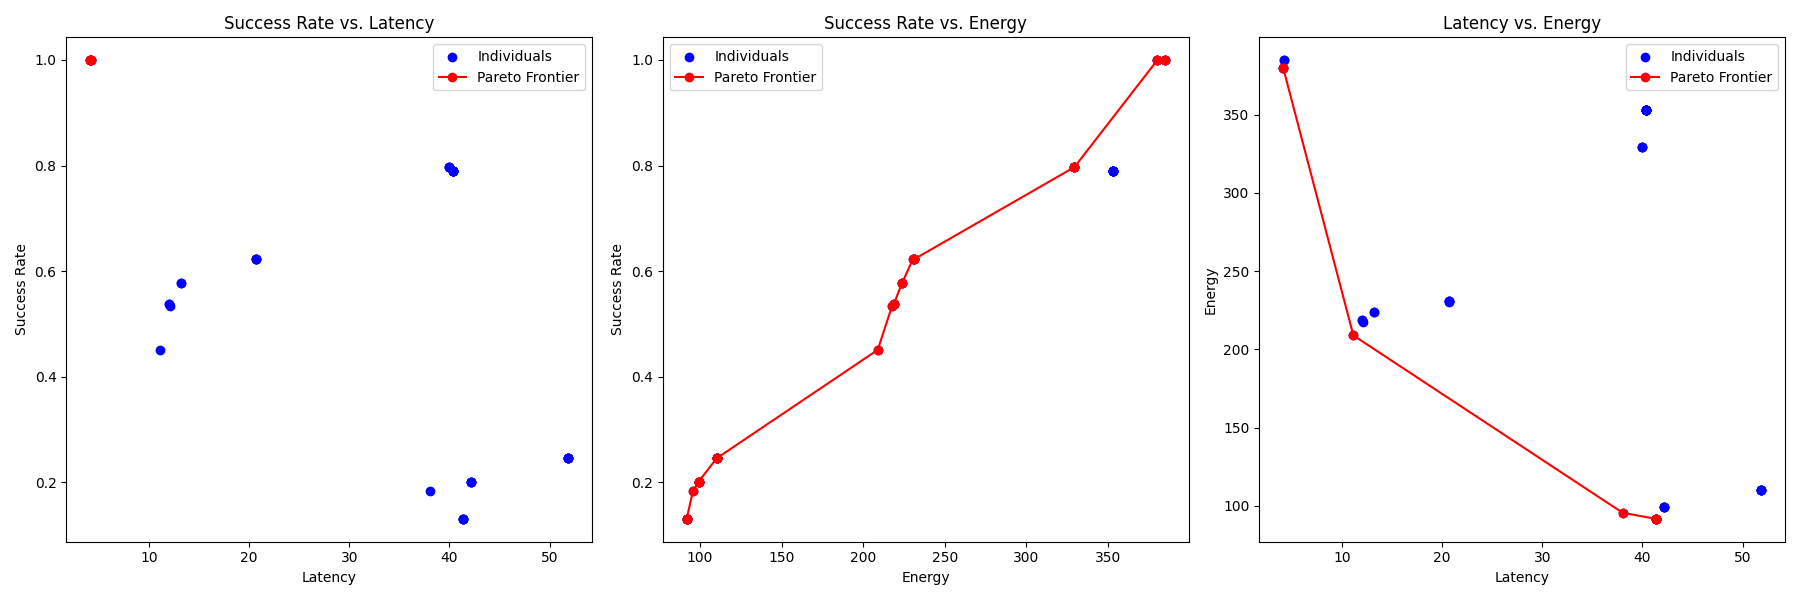
\includegraphics[width=0.9\linewidth]{figs/pareto_frontiers_nsga2.png}
    \caption{Pareto Frontiers Discovered by NSGA2 (MLP Genome)}
    \label{fig:nsga2-pareto-frontiers}
\end{figure}

\begin{figure}[H]
    \centering
    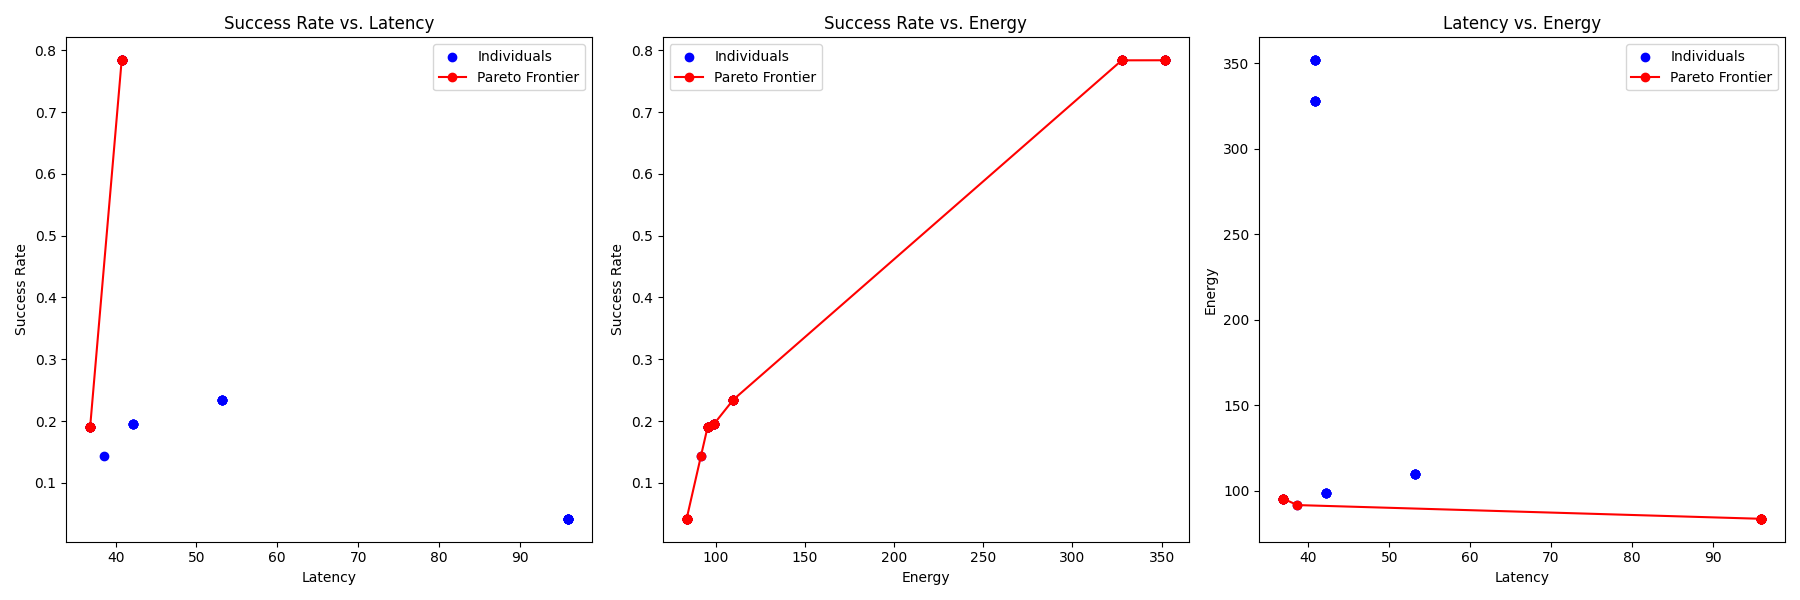
\includegraphics[width=0.9\linewidth]{figs/pareto_frontiers_npga.png}
    \caption{Pareto Frontiers Discovered by NPGA (MLP Genome)}
    \label{fig:npga-pareto-frontiers}
\end{figure}

\paragraph{Why GA Is Not Considered for Transformers}
Given the high dimensionality of Transformer parameters (approximately 350k), evolutionary algorithms would face immense difficulty converging within reasonable time and computational budgets. Hence, the DQL approach is used for Transformer-based models, exploiting gradient descent to handle large parameter counts more efficiently.

\paragraph{Discussion}
The comparative analysis reveals distinct advantages and limitations for each approach. The genetic algorithm demonstrates superior capability in generating a diverse range of Pareto-optimal solutions, thereby providing greater flexibility in objective weighting and multi-criteria optimization scenarios. In contrast, the deep Q-reinforcement learning approach exhibits faster convergence characteristics, rapidly converging to a single high-quality policy when hyperparameters are appropriately configured, while demonstrating reduced sensitivity to initial random seed selection. However, both methodologies present notable limitations that warrant consideration. The GA-based training approach incurs significant computational overhead, potentially limiting its applicability in resource-constrained environments. Conversely, the DQL framework is susceptible to local optima entrapment when learning rates or exploration parameters are suboptimally configured, which can substantially compromise solution quality and training stability.

\section{Conclusion and Perspectives}\label{sec:conclusion}

In the context of hierarchical edge-fog-cloud computing environments, this study has presented a new realistic offloading scenario based on real IoT task traces and a heterogeneous network topology. 
NOTE and T-NOTE architectures were proposed to address the complex task offloading problem, leveraging the strengths of Transformer encoder models. The performance of these architectures was evaluated against a baseline greedy approach and MLP-based DQL, outperforming them on all key metrics, including latency, task through rate (TTR), and energy consumption. -GA

Future research directions include exploring other optimization algorithms based on the environment state such as actor-critic methods (A2C, DDPG, PPO). Additionally, a more extensive study on multi objectives GA-based methods could be conducted to validate their effectiveness for this problem.


 \bibliographystyle{elsarticle-harv} 
 \bibliography{references}

\end{document}

\endinput



